\documentclass[11pt]{article}

\usepackage[margin=1in]{geometry}
\usepackage{amsmath,amssymb}
\usepackage{booktabs}
\usepackage{array}
\usepackage{graphicx}
\usepackage{tikz}
\usetikzlibrary{positioning,arrows.meta,shapes.geometric,calc}
\usepackage{natbib}
\usepackage{hyperref}
\usepackage{xcolor}
\usepackage{caption}
\usepackage{float}
\usepackage{fancyhdr}
\usepackage{lastpage}
\usepackage{bookmark}
\usepackage{needspace}
\numberwithin{equation}{section}

\definecolor{lemmaNavy}{HTML}{16324F}
\definecolor{lemmaBlue}{HTML}{2D6A9F}
\definecolor{lemmaGreen}{HTML}{2F7D5C}
\definecolor{lemmaWarm}{HTML}{A55B2A}
\captionsetup{font=small,labelfont={bf,color=lemmaNavy},labelsep=period}
\setlength{\textfloatsep}{16pt plus 3pt minus 3pt}
\setlength{\intextsep}{14pt plus 3pt minus 3pt}
\setlength{\abovecaptionskip}{7pt}
\setlength{\belowcaptionskip}{0pt}
\pagestyle{fancy}
\fancyhf{}
\lhead{\small\textsc{LEMMA}}
\rhead{\small Saxena and Kharat}
\cfoot{\small\thepage\ / \pageref{LastPage}}
\renewcommand{\headrulewidth}{0.3pt}
\renewcommand{\footrulewidth}{0pt}
\clubpenalty=10000
\widowpenalty=10000
\displaywidowpenalty=10000
% Keep normal paragraph pagination. A blanket interline penalty forces whole paragraphs onto
% the next page around floats, creating large empty regions without improving readability.
\interlinepenalty=0

\hypersetup{
  colorlinks=true,
  linkcolor=lemmaNavy,
  citecolor=lemmaBlue,
  urlcolor=lemmaBlue,
  pdftitle={LEMMA: Learned Guidance for Evidence-Carrying Long-Horizon Symbolic Rewriting},
  pdfauthor={Atul Saxena; Pushp Kharat},
  pdfsubject={Neuro-symbolic search-guided symbolic rewriting; goal-conditioning ablation; verified rewrite systems},
  pdfkeywords={neuro-symbolic, Monte Carlo tree search, symbolic rewriting, verified computation, goal conditioning},
  pdflang={en-US}
}

\title{\textbf{LEMMA: Learned Guidance for Evidence-Carrying\\ Long-Horizon Symbolic Rewriting}}
\author{%
\begin{tabular}{c@{\hspace{18mm}}c}
\textbf{Atul Saxena} & \textbf{Pushp Kharat} \\
\small\href{mailto:atul@blackdrome.tech}{atul@blackdrome.tech} & \small\href{mailto:pushp@pkboost.co.in}{pushp@pkboost.co.in} \\
\small BlackdromeAI Labs & \small Pkboost AI Labs
\end{tabular}}
\date{September 2026\\[-1mm]\small\textit{With contributions from Divyanshi Sharma, BlackdromeAI Labs}\quad\href{mailto:divyanshi@blackdrome.tech}{divyanshi@blackdrome.tech}}

\newcommand{\lemma}{\textsc{Lemma}}
\newcommand{\good}{89}

\begin{document}
\maketitle
\thispagestyle{plain}
\begin{center}
\small\textsc{Open resources}\quad
\href{https://github.com/blackdromeai-labs/LEMMA}{Code repository}
\;{\color{lemmaNavy}\textbar}\;\href{https://huggingface.co/datasets/BlackdromeAILabs/lemma-long-horizon-rewrite-benchmark}{Benchmark dataset}
\;{\color{lemmaNavy}\textbar}\;\href{https://huggingface.co/BlackdromeAILabs/lemma-v3-policy}{Released v3 model}
\;{\color{lemmaNavy}\textbar}\;\href{https://doi.org/10.5281/zenodo.22842820}{Paper DOI}
\end{center}
\vspace{-2mm}

\begin{abstract}
Symbolic mathematics systems can often verify an individual algebraic rewrite cheaply. The harder problem is selecting a long sequence of valid rewrites that transforms a starting expression into a specified goal. This becomes difficult when an intermediate expression has several verifier-admitted moves, because a locally plausible choice can lead away from the target. \lemma{} is a neuro-symbolic system built for this setting. It combines a Rust symbolic rule engine with a guardrail that filters candidate actions, an evidence-typed verifier that checks every accepted transition, and a neural policy that ranks the remaining choices. The design separates two questions that are often conflated: which transformations are valid, and which valid transformation is most useful for reaching the goal. Each returned derivation also carries an explicit symbolic, numerical, or replay-only evidence status.

We evaluate six search and decoding procedures on a frozen 120-problem long-horizon benchmark, with reference derivations of depths 64, 96, and 128. Eighty-nine problems contain genuine decision points rather than forced rewrite corridors. All methods receive the same guardrail-filtered, verifier-admitted successors, allowing the experiment to isolate the contribution of learned guidance. Uniform MCTS and value-only MCTS solve none of these 89 problems. At a 400 generated-successor budget, width-8 beam search also solves none, although it reaches all 89 when its budget increases to 1600. In contrast, policy--value MCTS solves 61/89, policy-only MCTS solves 87/89, and greedy decoding with the learned policy solves all 89/89 without tree search.

These results show that, on this controlled benchmark, learned local action ranking is the most budget-efficient component of the system. We additionally report a matched three-seed target-conditioning study, analyze the present value head, and release the complete experimental harness so that the reported derivations and evaluation protocol can be reproduced.
\end{abstract}

\section{Introduction}

Symbolic computer algebra systems can check an individual rewrite cheaply. The hard part is choosing a sequence of rewrites that reaches a particular target. For small expressions, brute force or a hand-written heuristic is usually enough. It is not enough when a derivation needs dozens of correct choices and each state has several legal moves. In the branching regime studied here, exhaustive search grows exponentially with depth even though individual steps remain cheap to check.

\lemma{} couples a Rust rule engine with a guardrail that removes implausible actions, an evidence-typed verifier, and learned action guidance. We evaluate greedy decoding, beam search, and PUCT-style MCTS over the same verifier-admitted successors. Each reported derivation is replayed against the live rule engine and retains its evidence status (Section~\ref{sec:kernel}). Numerical checks use bounded sampling, so they provide evidence rather than a proof certificate.

The paper has four contributions.

\textbf{First}, we implement a verifier-constrained neuro-symbolic rewriting system: learned components rank only guardrail-filtered, verifier-accepted actions, and every returned derivation carries explicit evidence provenance.

\textbf{Second}, we introduce a controlled 120-problem, long-horizon evaluation at depths 64--128. Each reference path is replayed exactly and each state's branching factor is measured directly. On the 89 problems with genuine choices, greedy learned decoding solves all 89, policy-only MCTS solves 87, and policy--value MCTS solves 61; uniform and value-only MCTS solve none. Width-8 beam search rises from 0/89 at budget 400 to 89/89 at budget 1600. This controlled component comparison is the central empirical result.

\textbf{Third}, a six-way decision-procedure comparison and beam-budget curve identify learned action priors as the most budget-efficient component: greedy policy execution solves all 89 branching problems, while beam requires a fourfold larger generated-successor budget to do the same.

\textbf{Fourth}, we measure verified branching at every state in every reference solution, separating forced corridors from genuinely decision-bearing cases.

The scope is deliberately narrow. We do not claim state-of-the-art mathematical reasoning or compare against computer algebra systems and theorem provers on their own benchmarks. The rule vocabulary covers seventeen algebraic, trigonometric, and linear-equation template families (Table~\ref{tab:rules}), and evaluation uses an expert-reviewed, purpose-built controlled benchmark rather than an external general-mathematics leaderboard. Within this setting, the ablation identifies learned local action ranking as the most budget-efficient component. The current value head does not improve on direct policy execution, while beam search reaches the same endpoint only at a substantially larger budget.

\section{Related Work}

\textbf{Symbolic computation and learned symbolic mathematics.} General-purpose computer algebra systems such as SymPy \citep{sympy2017} apply a fixed library of simplification and solving procedures under hand-tuned heuristics rather than learned search; \lemma{}'s rule engine and verifier occupy a similar role as a trusted, checkable substrate, but the question this paper asks is upstream of that substrate: given a correct set of rules, how does a system decide \emph{which} one to apply at each of many steps. A separate line of work trains a sequence model to emit a symbolic result directly, with no verified intermediate derivation: transformers that predict an integral or ODE solution in one shot \citep{lample2020symbolic}, that compute linear-algebra operations end to end \citep{charton2022linear}, that regress a closed-form recurrence from data \citep{dascoli2022symbolic}, that synthesize and execute an external program \citep{drori2022neural}, or that are scored purely on final-answer match with no notion of a checkable step at all \citep{saxton2019mathematics}. \citet{davies2021advancing} instead uses a trained model's attributions to guide a human toward a conjecture, with verification happening entirely outside the system as subsequent human proof. None of these commits to a sequence of independently verified rewrite steps toward a specified target expression, which is the setting \lemma{} is built for.

\textbf{Term rewriting, rewrite strategies, and equality saturation.} Classical term-rewriting theory \citep{knuthbendix1970,dershowitz1987termination,baadernipkow1998term,terese2003term} establishes confluence and termination for a rule \emph{set} offline, once; \lemma{} sidesteps a termination proof entirely, instead bounding search depth and empirically validating each benchmark path via replay. Strategy languages such as Stratego \citep{visser2001stratego} and rewriting-logic engines such as Maude \citep{clavel2002maude} occupy the same architectural slot as \lemma{}'s policy network, controlling which rule fires and in what order, but with a hand-written rather than learned strategy. Equality saturation \citep{tate2009equality,egg2021} takes a different approach to the same underlying search problem: rather than committing to one path, it represents many equivalent forms simultaneously via an e-graph and extracts a best one by cost function once no more rewrites apply, which sidesteps path selection at the cost of scaling with the union of all reachable forms rather than one path's length; \lemma{} instead commits to a policy-guided path, the more natural choice when the goal is one specific target expression rather than an unconstrained "best" form. \citet{nandi2021ruler} uses equality saturation to \emph{synthesize} a rewrite-rule set automatically, a different point on the "what is learned" axis than \lemma{}, whose seventeen template families are hand-authored and only ever selected among.

\textbf{Neural-guided theorem proving.} AlphaZero \citep{silver2018alphazero} established self-play MCTS guided by a joint policy-value network as a general search recipe; \lemma{}'s search layer descends from this design, adapted to verified rewriting rather than a two-player game. GPT-f \citep{polu2020gptf} and HyperTree Proof Search \citep{lample2022htps} apply this family of ideas to Metamath, Lean, and a purpose-built equation environment via online training from the prover's own search traces. HTPS reports the same qualitative pattern this paper does: trained guidance separates solving from not solving at depth while search alone contributes little. AlphaProof \citep{hubert2025alphaproof} scales the recipe to olympiad mathematics via large-scale auto-formalization and test-time reinforcement learning. A parallel, tactic-level branch of this literature operates over an interactive theorem prover's full proof state and its accessible theorem library rather than a single expression: TacticToe \citep{gauthier2021tactictoe} and TacticZero \citep{wu2021tacticzero} learn tactic selection in HOL4, the former from human proof corpora with MCTS and the latter tabula rasa by reinforcement learning with explicit backtracking; HOList and DeepHOL-Zero \citep{bansal2019holist,bansal2019deephol} search a large, open premise library in HOL Light; CoqGym \citep{yang2019coqgym}, PACT \citep{han2021pact}, Thor \citep{jiang2022thor}, LeanDojo \citep{yang2023leandojo}, Baldur \citep{first2023baldur}, and LISA \citep{jiang2021lisa} span Coq, Lean, and Isabelle with tactics ranging from single steps to whole-proof generation. In every case, the action is a tactic call, often itself a sub-search or a call to an external hammer, over an open theorem library, and correctness is checked by a general-purpose prover's trusted kernel; \lemma{} instead selects among a small, guardrail-filtered set of rewrites on one expression, checked by a bespoke evidence-typed verifier, which is what makes a controlled, matched-pairs ablation of a single architectural choice (goal-conditioning, Section~\ref{sec:ablation}) tractable in a way it is not on top of an open-ended proof library.

\textbf{Certifying algorithms and skeptical computation.} \lemma{}'s guardrail-and-verifier split is an instance of a much older proposer/checker separation. Result checking \citep{blum1995designing} and certifying algorithms \citep{mcconnell2011certifying} formalize a cheap, independent checker that certifies an output without trusting the computation that produced it; \citet{alkassar2014framework} goes further and machine-verifies, in Isabelle/HOL, that such a checker is itself correct. This is a strictly stronger guarantee than \lemma{}'s verifier, whose symbolic checks rest on a trusted but unverified implementation and whose numerical checks are explicitly non-exhaustive sampling (Table~\ref{tab:evidence}). \citet{harrison1998skeptic} pairs Maple (search) with HOL (independent re-derivation) in what is architecturally the closest historical analogue to \lemma{}'s own split, decades before any learned component; \citet{kaliszyk2007certified} and \citet{thery2001buchberger} instead build correctness in \emph{by construction} inside a proof assistant, the opposite trust model from \lemma{}'s check-after-proposal. \citet{harrison2008formal} supplies the vocabulary this paper's own distinction between "traceability of evidence" and "a proof certificate" (Section~\ref{sec:evidence}) draws on directly.

\textbf{Neuro-symbolic mathematical systems.} Concurrent with this work, \citet{xie2026mathesis} proposes a neuro-symbolic architecture pairing a hypergraph-based symbolic reasoning kernel with a transformer policy under an energy-guided objective, searched with MCTS and an evolutionary variant; the overall shape, a verified symbolic core beneath a learned policy beneath search, is the one \lemma{} adopts, and this paper's contribution is empirical rather than architectural: a controlled measurement of what that learned policy actually needs to see. AlphaGeometry \citep{trinh2024alphageometry} pairs a language model with a symbolic deduction engine the model calls on when deduction alone stalls, verified by exact symbolic deduction throughout, on a 30-problem olympiad-geometry benchmark. FunSearch and AlphaEvolve \citep{romeraparedes2024funsearch,novikov2025alphaevolve} evolve candidate programs with an LLM as mutation operator and a deterministic evaluator as the only correctness signal, an evolutionary loop with no tree search or learned value estimate, targeting open-ended constructions rather than one fixed goal expression. Peano \citep{poesia2023peano} defines a dependently-typed environment with a finite legal-action set at each state, close in spirit to \lemma{}'s guardrail, but verifies by type-checking over a general proof system rather than symbolic-or-sampled-numerical evidence over a fixed rule vocabulary. \citet{qin2021nssolver} injects symbolic constraints as differentiable auxiliary losses for math-word-problem solving, a "symbolic" component with no independent, non-differentiable checker analogous to \lemma{}'s verifier.

Tables~\ref{tab:comparison-provers} and~\ref{tab:comparison} summarize where \lemma{} sits relative to the named systems discussed above, by learned guidance, search procedure, and verification.

\begin{table}[htbp]
\centering
\small
\begin{tabular}{@{}p{3.4cm}p{3.6cm}p{3.6cm}p{3.6cm}@{}}
\toprule
System & Learned guidance & Search & Verification \\
\midrule
SymPy \citep{sympy2017} & none & none (fixed procedure) & none (trusted implementation) \\
Equality saturation \citep{tate2009equality,egg2021} & none & e-graph saturation, no path search & none (extraction by cost function) \\
AlphaZero \citep{silver2018alphazero} & policy + value network & MCTS (self-play) & game rules, not a proof kernel \\
GPT-f \citep{polu2020gptf} & tactic-prediction policy & best-first proof search & Metamath kernel \\
HTPS \citep{lample2022htps} & policy + value network & MCTS (hypertree), online training & Lean / Metamath / Equations kernel \\
AlphaProof \citep{hubert2025alphaproof} & policy + value network, test-time RL & MCTS & Lean kernel \\
TacticToe \citep{gauthier2021tactictoe} & tactic-selection policy (from human proofs) & MCTS, open tactic library & HOL4 kernel \\
TacticZero \citep{wu2021tacticzero} & tactic policy, tabula rasa RL & RL rollout with explicit backtracking & HOL4 kernel \\
LeanDojo / ReProver \citep{yang2023leandojo} & retrieval-augmented tactic policy & best-first search over $\sim$100K-theorem library & Lean kernel \\
\bottomrule
\end{tabular}
\caption{Symbolic-rewriting and theorem-proving systems, one row per named system rather than merged by family, since kernel and training source differ across them even within a family. Target-conditioning and evidence granularity are discussed in prose above; every system here is target-conditioned (a specific theorem statement) except the first two.}
\label{tab:comparison-provers}
\end{table}

\begin{table}[htbp]
\centering
\small
\begin{tabular}{@{}p{3.4cm}p{3.6cm}p{3.6cm}p{3.6cm}@{}}
\toprule
System & Learned guidance & Search & Verification \\
\midrule
AlphaGeometry \citep{trinh2024alphageometry} & language model (auxiliary constructions) & symbolic deduction engine, not MCTS & exact symbolic deduction \\
FunSearch / AlphaEvolve \citep{romeraparedes2024funsearch,novikov2025alphaevolve} & LLM as mutation operator & evolutionary loop, no tree search & deterministic evaluator \\
Peano \citep{poesia2023peano} & policy over typed actions & search over dependent-type environment & type-checking \\
Mathesis \citep{xie2026mathesis} & energy-guided transformer policy & MCTS + evolutionary variant & symbolic reasoning kernel \\
\lemma{} \textbf{(this paper)} & goal-conditioned policy + value network & MCTS (PUCT) & bespoke evidence-typed verifier (Table~\ref{tab:evidence}) \\
\bottomrule
\end{tabular}
\caption{Neuro-symbolic, evolutionary, and typed-environment systems, and where \lemma{} sits among them. FunSearch/AlphaEvolve target open-ended constructions rather than a fixed goal; the other four, including \lemma{}, condition on a specific target.}
\label{tab:comparison}
\end{table}

\section{System: The Symbolic Kernel}
\label{sec:kernel}

Every rewrite \lemma{} performs passes through three layers before it is accepted, shown in Figure~\ref{fig:pipeline}. Given the current expression, a lightweight \emph{guardrail} first restricts the set of rules worth attempting: it profiles the expression's shape and returns only the rules whose preconditions could plausibly apply, which keeps the branching factor the search actually faces close to the branching factor a human would recognize, rather than the full library of several hundred registered rules. The \emph{rule engine} then applies each guardrail-admitted rule and produces candidate successor expressions. Finally, an \emph{evidence-typed verifier} checks every candidate: symbolic equivalence where a closed-form check exists, and otherwise numerical evaluation at multiple sampled points under a seeded random generator, so that a candidate step is either accepted with an explicit type of evidence attached or rejected outright. A step that is not verifier-accepted is never presented to the search layer as an option, regardless of what the rule engine produced.

More formally, let $\mathcal{G}(s)$ be the actions admitted by the guardrail at state $s$, let $T_a(s)$ be the successor proposed by action $a$, and let $V(s,T_a(s))$ denote the verifier's result. Search receives only the following finite action set:
\begin{equation}
\mathcal{A}(s)=\{a\in\mathcal{G}(s) : T_a(s)\neq s\ \land\ V(s,T_a(s))\in\{\textsc{Symbolic},\textsc{Numeric},\textsc{Replay}\}\}.
\label{eq:legal-actions}
\end{equation}
The non-identity condition prevents a rule from creating a vacuous self-loop. Equation~\eqref{eq:legal-actions} is the boundary between symbolic execution and learned search: the network ranks admissible actions, but it cannot make an inadmissible one available.

\begin{figure}[H]
\centering
\resizebox{0.94\textwidth}{!}{%
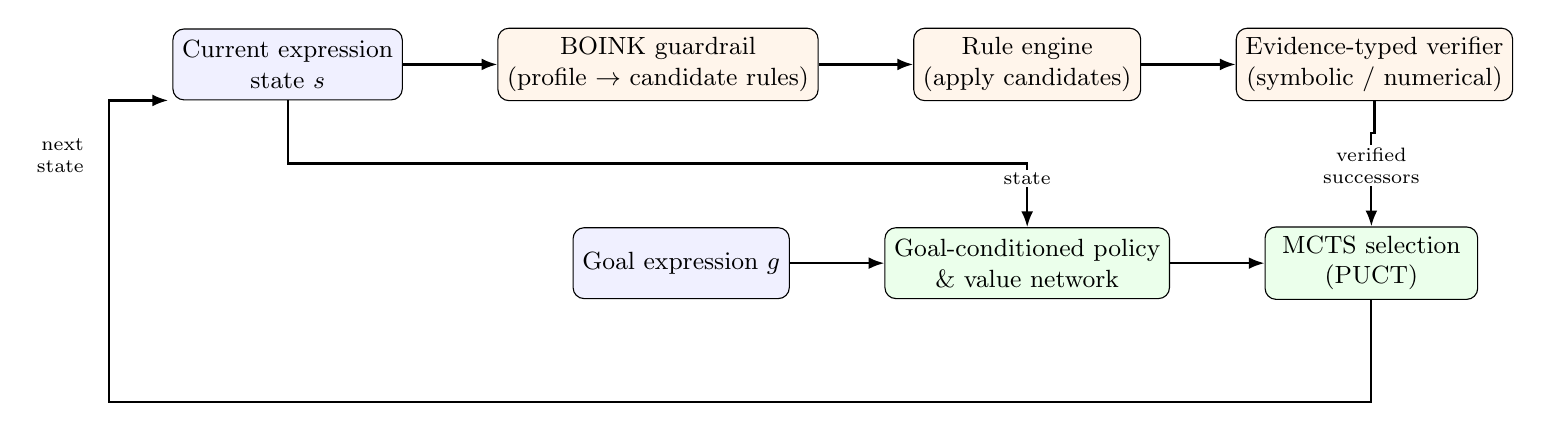
\begin{tikzpicture}[
  node distance=8mm and 12mm,
  box/.style={draw, rounded corners, minimum height=9mm, minimum width=27mm, align=center, font=\small},
  arr/.style={-{Latex[length=2mm]}, thick}
]
\node[box, fill=blue!6] (state) {Current expression\\state $s$};
\node[box, right=of state, fill=orange!8] (guard) {BOINK guardrail\\(profile $\to$ candidate rules)};
\node[box, right=of guard, fill=orange!8] (rules) {Rule engine\\(apply candidates)};
\node[box, right=of rules, fill=orange!8] (verify) {Evidence-typed verifier\\(symbolic / numerical)};
\node[box, below=16mm of rules, fill=green!8] (policy) {Goal-conditioned policy\\\& value network};
\node[box, left=of policy, fill=blue!6] (goal) {Goal expression $g$};
\node[box, right=of policy, fill=green!8] (mcts) {MCTS selection\\(PUCT)};

\coordinate (vDrop) at ($(verify.south)+(0,-4mm)$);
\coordinate (stateDrop) at ($(state.south)+(0,-8mm)$);
\coordinate (mctsDrop) at ($(mcts.south)+(0,-13mm)$);

\draw[arr] (state) -- (guard);
\draw[arr] (guard) -- (rules);
\draw[arr] (rules) -- (verify);
\draw[arr] (goal) -- (policy);
\draw[arr] (policy) -- (mcts);

\draw[arr] (verify.south) -- (vDrop) -| (mcts.north);
\node[font=\scriptsize, align=center, above=5mm of mcts.north, fill=white, inner sep=1pt] {verified\\successors};

\draw[arr] (state.south) -- (stateDrop) -| (policy.north);
\node[font=\scriptsize, above=5mm of policy.north, fill=white, inner sep=1pt] {state};

\coordinate (returnEntry) at ($(state.south west)+(-8mm,0)$);
\draw[arr, shorten >=1.5pt] (mcts.south) -- (mctsDrop) -- (returnEntry |- mctsDrop) -- (returnEntry) -- (state.south west);
\node[font=\scriptsize, align=right, anchor=east] at ([xshift=-2mm,yshift=-7mm]returnEntry) {next\\state};
\end{tikzpicture}%
}
\caption{One iteration of \lemma{}'s search loop. The guardrail, rule engine, and verifier form a trusted pipeline that only ever exposes verified successor states to the search layer; the policy and value network is conditioned on both the current state and the fixed goal expression, and its output only ranks moves the verifier has already accepted.}
\label{fig:pipeline}
\end{figure}

This ordering is deliberate: the guardrail is a performance filter, not a correctness gate, so the verifier is the last word on whether a step is legitimate, and the policy network never gets an opportunity to rank a move the verifier would have rejected. Training data generation reuses this exact pipeline. The same guardrail-then-verifier filter used at inference time enumerates legal actions during data generation, so the model is never trained on moves the real search could not itself take.

\subsection{Evidence status}
\label{sec:evidence}

"Verified" is not one thing in \lemma{}; it is one of five whole-trace statuses, each built from per-step evidence of one of three strengths (Table~\ref{tab:evidence}). A step is checked by \emph{symbolic equivalence} when both sides reduce to the same canonical form, the strongest check available, though still an equivalence check rather than a machine-checked soundness proof of the rule itself. Where no closed-form check applies, the verifier falls back to \emph{numeric sampling}: both sides are evaluated at multiple points under a seeded generator and compared, which is evidence, not proof, since sampling can miss a disagreement at an unsampled point. A third, weaker method, \emph{rule replay only}, applies where the expression contains a derivative or integral the evaluator cannot sample; it confirms the step reproduced the rule's own claimed output, not that the rule is sound. Figure~\ref{fig:trust} shows how a single proposed step is classified, and how per-step evidence combines into the whole-trace status this paper reports for a solution.

\begin{table}[htbp]
\centering
\small
\begin{tabular}{@{}ll>{\raggedright\arraybackslash}p{7.6cm}@{}}
\toprule
Level & Status & Acceptance semantics \\
\midrule
per-step & Symbolic equivalence & Both sides reduce to the same canonical form. \\
 & Numeric sampling & Both sides agree at every sampled point; evidence, not proof. \\
 & Rule replay only & Re-running the rule reproduced its claimed output; nothing further checked (derivatives/integrals). \\
\midrule
whole-trace & Checked & Replays end to end; every step independently checked (symbolic or numeric), none by replay-only. \\
 & Partial & Replays; at least one step is weaker than the rest (a replay-only step, or a mix of symbolic and numeric). \\
 & Heuristic & Replays; every step relies on the weaker methods throughout (all numeric, or all replay-only). \\
 & Unverified & Does not replay end to end, or contains an unchecked step. \\
 & Unsupported & The requested verification mode is not implemented for this case. \\
\bottomrule
\end{tabular}
\caption{The evidence taxonomy \lemma{} actually implements (\texttt{mm-verifier::status}). Only \texttt{Checked} is reported as fully verified; every other status is retained and shown, not silently upgraded. All results in Section~\ref{sec:results} come from replayed, \texttt{Checked} or \texttt{Partial} traces; the corpora never contain a derivative or integral, so \texttt{Heuristic} via replay-only does not arise in this paper's experiments.}
\label{tab:evidence}
\end{table}

\begin{figure}[htbp]
\centering
\resizebox{0.96\textwidth}{!}{%
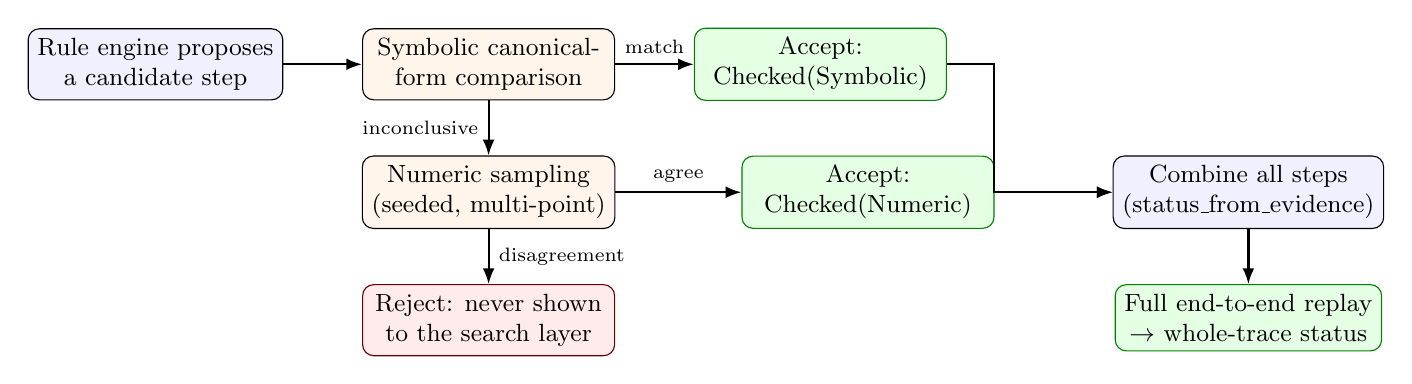
\begin{tikzpicture}[
  node distance=7mm and 10mm,
  box/.style={draw, rounded corners, minimum height=8mm, minimum width=32mm, align=center, font=\small},
  arr/.style={-{Latex[length=2mm]}, thick}
]
\node[box, fill=blue!6] (propose) {Rule engine proposes\\a candidate step};
\node[box, right=of propose, fill=orange!8] (symb) {Symbolic canonical-\\form comparison};
\node[box, below=of symb, fill=orange!8] (num) {Numeric sampling\\(seeded, multi-point)};
\node[box, right=of symb, fill=green!10, draw=green!50!black] (acc1) {Accept:\\Checked(Symbolic)};
\node[box, right=16mm of num, fill=green!10, draw=green!50!black] (acc2) {Accept:\\Checked(Numeric)};
\node[box, below=of num, fill=red!8, draw=red!40!black] (rej) {Reject: never shown\\to the search layer};
\node[box, right=15mm of acc2, fill=blue!6] (combine) {Combine all steps\\(status\_from\_evidence)};
\node[box, below=of combine, fill=green!10, draw=green!50!black] (final) {Full end-to-end replay\\$\to$ whole-trace status};

\draw[arr] (propose) -- (symb);
\draw[arr] (symb) -- node[above,font=\scriptsize]{match} (acc1);
\draw[arr] (symb) -- node[left,font=\scriptsize]{inconclusive} (num);
\draw[arr] (num) -- node[above,font=\scriptsize]{agree} (acc2);
\draw[arr] (num) -- node[right,font=\scriptsize]{disagreement} (rej);
\draw[arr] (acc1.east) -- ++(6mm,0) |- (combine.west);
\draw[arr] (acc2) -- (combine);
\draw[arr] (combine) -- (final);
\end{tikzpicture}%
}
\caption{Trust boundary for one proposed step, and how per-step evidence becomes the whole-trace status of Table~\ref{tab:evidence}. A rejected step never reaches the search layer as an option (Section~\ref{sec:kernel}); an accepted trace is only reported as a solution after a full end-to-end replay from the original input to the final output.}
\label{fig:trust}
\end{figure}

\section{The Neural Policy and Value Network}
\label{sec:network}

The network is a small transformer (embedding dimension 256, hidden dimension 512, 8 attention heads, 4 layers) with a token vocabulary of 64 symbols. It is sized for this task rather than adapted from a general-purpose language model. A recursive-descent tokenizer maps the current state $s$ and target $g$ to the goal-conditioned sequence
\begin{equation}
x(s,g)=[\texttt{START}]\;\operatorname{tok}(s)\;[\texttt{SEP}]\;\operatorname{tok}(g)\;[\texttt{END}].
\label{eq:input-encoding}
\end{equation}
The separator reuses a vocabulary slot that earlier versions of the encoder left unassigned. No tensor shape changed when goal conditioning was added, so previously trained state-only checkpoints remain loadable. Figure~\ref{fig:architecture} shows the complete forward pass.

For a padded batch, $m_i\in\{0,1\}$ marks a real token. If $H^{(0)}=E(x)+P$ is the token-plus-position representation and $F_\ell$ is transformer block $\ell$, the pooled representation is
\begin{equation}
H^{(\ell+1)}=F_\ell\!\left(H^{(\ell)};m\right),\qquad
z=\frac{\sum_{i=1}^{L}m_i H^{(4)}_i}{\sum_{i=1}^{L}m_i}.
\label{eq:masked-pooling}
\end{equation}
The same mask is added to the attention scores before softmax and used in the pooling denominator. Thus padded positions receive neither attention mass nor weight in $z$.

The policy head produces logits $\ell_a(s,g)$ for 572 rule actions plus a stop class. The value head returns $\hat v_\theta(s,g)=\tanh(w_v^\top z+b_v)\in[-1,1]$. At both training and inference, the action distribution is normalized only over the verifier-accepted set from Equation~\eqref{eq:legal-actions}:
\begin{equation}
\pi_\theta(a\mid s,g)=
\begin{cases}
\dfrac{\exp\!\left(\ell_a(s,g)\right)}{\sum_{b\in\mathcal{A}(s)}\exp\!\left(\ell_b(s,g)\right)}, & a\in\mathcal{A}(s),\\[2mm]
0, & a\notin\mathcal{A}(s).
\end{cases}
\label{eq:legal-policy}
\end{equation}

\begin{figure}[htbp]
\centering
\resizebox{0.98\textwidth}{!}{%
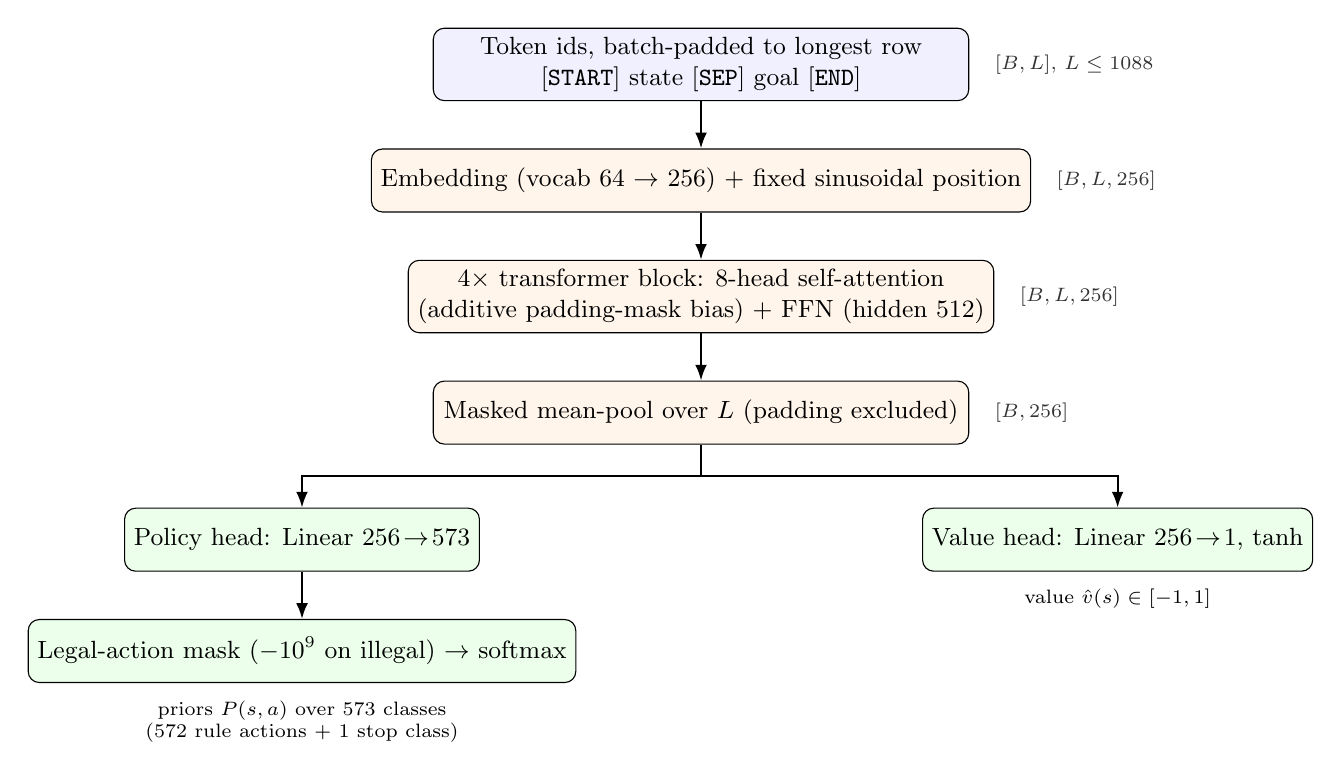
\begin{tikzpicture}[
  node distance=6mm,
  box/.style={draw, rounded corners, minimum height=8mm, minimum width=68mm, align=center, font=\small},
  shp/.style={font=\scriptsize, gray!40!black},
  arr/.style={-{Latex[length=2mm]}, thick}
]
\node[box, fill=blue!6] (tok) {Token ids, batch-padded to longest row\\$[\texttt{START}]$ state $[\texttt{SEP}]$ goal $[\texttt{END}]$};
\node[shp, right=2mm of tok] {$[B,L]$, $L\le 1088$};

\node[box, below=of tok, fill=orange!8] (emb) {Embedding (vocab 64 $\to$ 256) + fixed sinusoidal position};
\node[shp, right=2mm of emb] {$[B,L,256]$};

\node[box, below=of emb, fill=orange!8] (attn) {$4\times$ transformer block: 8-head self-attention\\(additive padding-mask bias) + FFN (hidden 512)};
\node[shp, right=2mm of attn] {$[B,L,256]$};

\node[box, below=of attn, fill=orange!8] (pool) {Masked mean-pool over $L$ (padding excluded)};
\node[shp, right=2mm of pool] {$[B,256]$};

\node[box, below left=8mm and -6mm of pool, fill=green!8, minimum width=42mm] (pol) {Policy head: Linear $256\!\to\!573$};
\node[box, below right=8mm and -6mm of pool, fill=green!8, minimum width=42mm] (val) {Value head: Linear $256\!\to\!1$, $\tanh$};

\node[box, below=6mm of pol, fill=green!8, minimum width=42mm] (mask) {Legal-action mask ($-10^9$ on illegal) $\to$ softmax};
\node[below=1mm of mask, font=\scriptsize, align=center] {priors $P(s,a)$ over 573 classes\\(572 rule actions + 1 stop class)};

\node[below=1mm of val, font=\scriptsize] {value $\hat v(s)\in[-1,1]$};

\draw[arr] (tok) -- (emb);
\draw[arr] (emb) -- (attn);
\draw[arr] (attn) -- (pool);
\draw[arr] (pool.south) -- ++(0,-4mm) -| (pol.north);
\draw[arr] (pool.south) -- ++(0,-4mm) -| (val.north);
\draw[arr] (pol) -- (mask);
\end{tikzpicture}%
}
\caption{The full forward pass, with tensor shapes ($B$ = batch, $L$ = sequence length). Both heads share every layer up to the pooled representation; the legal-action mask is applied identically at training time (inside the cross-entropy loss, Section~\ref{sec:training}) and at inference time (before PUCT reads the priors, Section~\ref{sec:search}), so the network never has an opportunity to prefer an action the symbolic pipeline has not already certified as legal.}
\label{fig:architecture}
\end{figure}

The encoder accepts each expression at its natural token length, or returns a typed error when the configured bound is exceeded. This matters for the long-horizon corpus: depth-8 inputs require 45 tokens, while depth-128 inputs require 531--615. Batches pad only to their longest row. An additive attention bias and a masked pooling denominator ensure that padding contributes neither to attention nor to the pooled representation; a regression test compares tight and padded encodings of the same expression and requires near-identical output.

A model's manifest records a single boolean, \texttt{goal\_conditioned}, and the search layer consults it before every policy or value query: a goal-conditioned model is never fed a state-only encoding, and a state-only model is never asked to condition on a goal it was not trained to use. This is enforced in code, not by convention, specifically so that the ablation in Section~\ref{sec:ablation} cannot be silently invalidated by the two arms being evaluated inconsistently.

\section{Training Procedure}
\label{sec:training}

Training examples are generated from a set of seventeen parametrized "core" templates (Table~\ref{tab:rules}): collecting like terms, constant folding, distributing a product over a sum, the difference-of-squares identity, zero-annihilation, the Pythagorean identity, sine-arcsine and cosine-arccosine cancellation, six families of equation-preserving cancellation, and three families in which only the goal (not the state) determines the correct move. Each template specifies a genuinely solvable start-to-goal pair together with the exact rule sequence connecting them. Table~\ref{tab:rules} lists every core family; four of the seventeen (\texttt{collect-like-terms}, \texttt{const-fold}, \texttt{distribute}, \texttt{zero-annihilation}) are used as the innermost solvable kernels in the benchmark (Section~\ref{sec:setup}). Several rules from other families, including \texttt{power\_of\_one}, \texttt{identity\_mul\_one}, \texttt{identity\_add\_zero}, and \texttt{double\_negative}, appear only as \emph{wrapper} motifs around those cores (Table~\ref{tab:branching}); the remaining thirteen families are exercised only during training.

\begin{table}[htbp]
\centering
\scriptsize
\resizebox{\textwidth}{!}{%
\begin{tabular}{@{}llll@{}}
\toprule
Core family & Representative rewrite & Rule key & In benchmark \\
\midrule
\texttt{collect-like-terms} & $ax+bx \to (a{+}b)x$ & \texttt{algebra::collect\_like\_terms} & as core \\
\texttt{const-fold} & $a+b \to (a{+}b)$ & \texttt{algebra::const\_fold} & as core \\
\texttt{distribute} & $a(x+b) \to ax+ab$ & \texttt{algebra::distribute} & as core \\
\texttt{difference-of-squares} & $x^2-b^2 \to (x{+}b)(x{-}b)$ & \texttt{algebra::difference\_of\_squares} & no \\
\texttt{zero-annihilation} & $0\cdot(ay+x) \to 0$ & \texttt{algebra::zero\_mul} & as core \\
\texttt{goal-decides-distribute} & $1\cdot(P{+}0) \to$ state \emph{or} distributed, by goal & \texttt{algebra::distribute} & no \\
\texttt{goal-decides-power-one} & $((x{+}a)^2)^1 \to (x{+}a)^2$, if goal selects it & \texttt{algebra::power\_of\_one} & as wrapper only \\
\texttt{goal-decides-power-mul} & $((x{+}a)^2)^1 \to (x{+}a)^{2\cdot1}$, if goal selects it & \texttt{algebra::power\_mul} & no \\
\texttt{pythagorean-identity} & $\sin^2(x{+}a)+\cos^2(x{+}a) \to 1$ & \texttt{trig::pythagorean\_identity} & no \\
\texttt{sin-arcsin} & $\sin(\arcsin(\sin x)) \to \sin x$ & \texttt{trig::sin\_arcsin} & no \\
\texttt{cos-arccos} & $\cos(\arccos(\cos y)) \to \cos y$ & \texttt{trig::cos\_arccos} & no \\
\texttt{equation-cancel-addition} & $x+a=b \to x=b-a$ & \texttt{equations::cancel\_addition} & no \\
\texttt{equation-cancel-subtraction} & $x-a=b \to x=b+a$ & \texttt{equations::cancel\_subtraction} & no \\
\texttt{equation-cancel-multiplication} & $ax=b \to x=b/a$ & \texttt{equations::cancel\_multiplication} & no \\
\texttt{equation-cancel-division} & $x/a=b \to x=ab$ & \texttt{equations::cancel\_division} & no \\
\texttt{equation-linear-solve} & $ax+b=c \to x=(c{-}b)/a$ & \texttt{equations::linear\_solve} & no \\
\texttt{equation-mixed-cancellation} & nested affine chain $\to x=$ solution & \texttt{equations::cancel\_*} (mixed) & no \\
\bottomrule
\end{tabular}%
}
\caption{Every core family in the training generator (\texttt{data\_deep.rs}). "In benchmark" marks whether the family's core problem (not merely one of its rules) appears in the frozen evaluation corpus; \texttt{power\_of\_one} is the one case where a family's rule appears in the benchmark only as a wrapper around a different core, not as its own core problem.}
\label{tab:rules}
\end{table}

Long problems are built by wrapping a core in "collision layers" (an identity transformation such as $1 \cdot (P+0)$, at which both the intended peeling move and an unrelated distribution move are simultaneously legal and verifier-accepted) and other one-step motifs, chosen so that the same three or four surface shapes cannot be memorized as a fixed prefix. Every candidate long problem is replayed against the real rule engine and verifier before being accepted; a construction that does not replay exactly onto its stated goal is discarded rather than relabeled. Figure~\ref{fig:datagen} traces this construction end to end, from one core template to the training rows a model actually optimizes against.

\begin{figure}[H]
\centering
\resizebox{0.98\textwidth}{!}{%
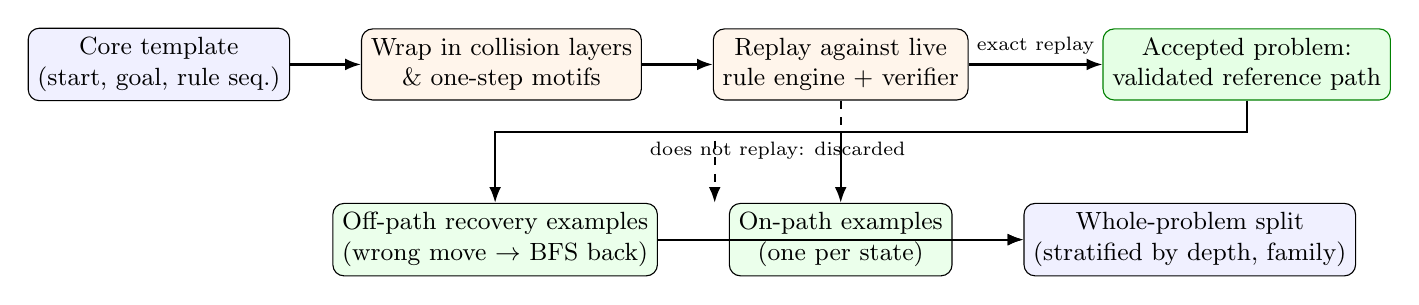
\begin{tikzpicture}[
  node distance=8mm and 9mm,
  box/.style={draw, rounded corners, minimum height=9mm, minimum width=27mm, align=center, font=\small},
  arr/.style={-{Latex[length=2mm]}, thick}
]
\node[box, fill=blue!6] (core) {Core template\\(start, goal, rule seq.)};
\node[box, right=of core, fill=orange!8] (wrap) {Wrap in collision layers\\\& one-step motifs};
\node[box, right=of wrap, fill=orange!8] (replay) {Replay against live\\rule engine + verifier};
\node[box, right=17mm of replay, fill=green!10, draw=green!50!black] (accept) {Accepted problem:\\validated reference path};

\node[box, below=13mm of replay, fill=green!8] (onpath) {On-path examples\\(one per state)};
\node[box, left=of onpath, fill=green!8] (recov) {Off-path recovery examples\\(wrong move $\to$ BFS back)};
\node[box, right=of onpath, fill=blue!6] (split) {Whole-problem split\\(stratified by depth, family)};

\draw[arr] (core) -- (wrap);
\draw[arr] (wrap) -- (replay);
\draw[arr] (replay) -- node[above,font=\scriptsize]{exact replay} (accept);
\draw[arr, dashed] (replay.south) -- ++(0,-4mm) -| node[pos=0.25,below,font=\scriptsize]{does not replay: discarded} ([xshift=-16mm]replay.south |- onpath.north);
\draw[arr] (accept.south) -- ++(0,-4mm) -| (onpath.north);
\draw[arr] (accept.south) -- ++(0,-4mm) -| (recov.north);
\draw[arr] (onpath) -- (split);
\draw[arr] (recov) -- (split);
\end{tikzpicture}%
}
\caption{Training-data construction. A construction that fails to replay exactly onto its stated goal is discarded, not relabeled (Section~\ref{sec:training}); the whole-problem, depth-and-family-stratified split at the end is what makes v1/v2/v3's held-out validation whole-problem rather than whole-state (Appendix~\ref{sec:v-lineage} discusses what this split does and does not test).}
\label{fig:datagen}
\end{figure}

One family, \texttt{goal-decides-distribute}, is included specifically because without it a policy can score well everywhere else while never actually consulting the goal: at the shape $1\cdot(P+0)$, every other family in the corpus answers "peel the identity," so a model can learn a shape-to-label mapping that ignores the goal entirely and still appear goal-conditioned by the encoding alone. \texttt{goal-decides-distribute} presents the identical shape with the opposite correct answer, forcing the label to depend on the goal rather than the state. We verify this property directly with a regression test before relying on it in the ablation.

Each training example has a verified legal-action set $\mathcal{A}(s)$ and a nonempty subset $\mathcal{R}(s,g)\subseteq\mathcal{A}(s)$ of actions that reach the reference successor. When several actions yield the same correct successor, the target does not arbitrarily choose one. It assigns them equal probability:
\begin{equation}
q(a\mid s,g)=
\begin{cases}
|\mathcal{R}(s,g)|^{-1}, & a\in\mathcal{R}(s,g),\\
0, & \text{otherwise}.
\end{cases}
\qquad
y(r)=2\cdot0.97^r-1,
\label{eq:targets}
\end{equation}
where $r$ is the number of reference steps remaining. The value target $y(r)$ gives the value head a monotone signal rather than a constant target.

The implemented objective combines legal-set cross-entropy with value regression, using the configured value weight $\lambda=0.5$:
\begin{equation}
\mathcal{L}(\theta)=-\sum_{a\in\mathcal{A}(s)}q(a\mid s,g)\log\pi_\theta(a\mid s,g)
+\lambda\left(\hat v_\theta(s,g)-y(r)\right)^2.
\label{eq:training-objective}
\end{equation}
Illegal logits receive a $-10^9$ mask before the log-softmax. They therefore receive neither policy probability nor gradient through the policy objective.

Some training runs additionally include off-path recovery data. From an on-path state, we take a legal but incorrect move and run bounded breadth-first search for a short return to the reference path. The policy therefore sees some examples of recovery after a wrong turn rather than only states on a correct solution. The recovery share is 13.4\% for v1, 3.5\% for v2, and 0\% for v3 and both ablation arms (Appendix~\ref{sec:v-lineage}).

Training uses AdamW, a cosine learning-rate schedule with warmup, and early stopping on a held-out whole-problem split stratified by depth and family. Each epoch's weights are saved to the primary output path; the released checkpoint is therefore the last epoch completed by that run. Appendix~\ref{sec:repro} records this selection rule alongside each arm's observed training duration.

\subsection{Seeded training protocol}
\label{sec:seed-bug}

Each training invocation receives an explicit \texttt{--seed}. The implementation reseeds the device generator and derives a separate seed for per-epoch batch ordering, while holding the generated data and its train/validation split fixed across a seed-matched comparison. A seed sweep therefore changes weight initialization and optimization trajectory, not the examples assigned to training or validation. Section~\ref{sec:ablation} uses this protocol for the paired target-conditioning study.

\section{Guided Search}
\label{sec:search}

Search is standard PUCT-style MCTS \citep{silver2018alphazero}, adapted so that a node's children are exactly the guardrail-filtered, verifier-accepted successors described in Section~\ref{sec:kernel}. It can never expand into a state the trusted pipeline would not itself certify. At a state $s$, selection chooses
\begin{equation}
a^*=\underset{a\in\mathcal{A}(s)}{\arg\max}\left[
Q(s,a)+c_{\mathrm{puct}}\,\pi_\theta(a\mid s,g)
\frac{\sqrt{N(s)}}{1+N(s,a)}
\right].
\label{eq:puct}
\end{equation}
Here $Q(s,a)$ is the running mean of backed-up values, $N(s)$ is the parent visit count, and $N(s,a)$ is the edge visit count. The implementation uses $c_{\mathrm{puct}}=1.41$ (Appendix~\ref{sec:repro}).

A newly reached leaf is expanded, evaluated by the value network, and backed up along the selected path. Goal states contribute a terminal value of $1$; nonterminal leaves contribute $\hat v_\theta(s,g)$. When the model is goal-conditioned, every policy and value query includes the fixed target expression. State-only models use the corresponding state-only calls, selected by the manifest flag from Section~\ref{sec:network}. Search stops on reaching the goal or exhausting its simulation budget, then returns the best path found and the number of expanded nodes.

Figure~\ref{fig:worked} shows one real, measured decision point rather than a schematic one. At step 32 of benchmark problem \texttt{deep-OOD-d64-001}, the current state has the shape $(\cdots)^2$ raised to the power $1$, at which two rules are simultaneously legal and verifier-accepted: \texttt{power\_of\_one} (peel the outer power, the reference-correct move) and \texttt{power\_mul} (multiply the two exponents instead, a legal but incorrect move, the \texttt{power\_of\_one}-family distractor in Table~\ref{tab:branching}). We queried model v3 (Appendix~\ref{sec:v-lineage}) at this exact state and goal; its raw priors are $0.0354$ for \texttt{power\_of\_one} against $6\times10^{-8}$ for \texttt{power\_mul}, renormalized to $100.0\%$ of the legal mass on the correct move. PUCT selects \texttt{power\_of\_one}; the verifier confirms the resulting step by symbolic canonical-form comparison (Section~\ref{sec:kernel}), the case for a definitional identity like this one, and search continues from the peeled state.

\begin{figure}[htbp]
\centering
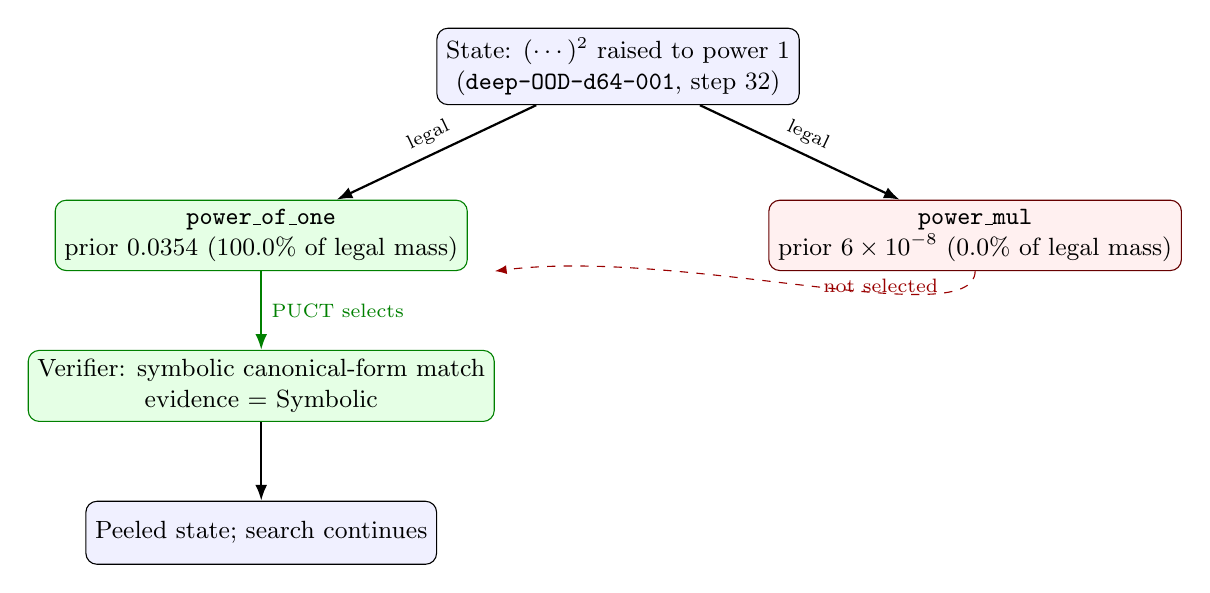
\begin{tikzpicture}[
  node distance=8mm and 10mm,
  box/.style={draw, rounded corners, minimum height=8mm, minimum width=38mm, align=center, font=\small},
  arr/.style={-{Latex[length=2mm]}, thick}
]
\node[box, fill=blue!6] (state) {State: $(\cdots)^2$ raised to power $1$\\(\texttt{deep-OOD-d64-001}, step 32)};

\node[box, below left=12mm and -4mm of state, fill=green!10, draw=green!50!black] (correct) {\texttt{power\_of\_one}\\prior $0.0354$ (100.0\% of legal mass)};
\node[box, below right=12mm and -4mm of state, fill=red!6, draw=red!40!black] (wrong) {\texttt{power\_mul}\\prior $6\times10^{-8}$ (0.0\% of legal mass)};

\node[box, below=10mm of correct, fill=green!10, draw=green!50!black] (verify) {Verifier: symbolic canonical-form match\\evidence = Symbolic};
\node[box, below=10mm of verify, fill=blue!6] (next) {Peeled state; search continues};

\draw[arr] (state) -- node[above,sloped,font=\scriptsize]{legal} (correct);
\draw[arr] (state) -- node[above,sloped,font=\scriptsize]{legal} (wrong);
\draw[arr, green!50!black, thick] (correct) -- node[right,font=\scriptsize]{PUCT selects} (verify);
\draw[arr] (verify) -- (next);
\draw[-{Latex[length=1.5mm]}, red!60!black, dashed] (wrong.south) .. controls +(0,-8mm) and +(2.4,3mm) .. (verify.east|-wrong.south) node[midway, right, font=\scriptsize, red!60!black, xshift=1mm] {not selected};
\end{tikzpicture}
\caption{A real, measured decision point: both rules are legal and verifier-accepted at this state, but the goal-conditioned policy's priors concentrate almost all mass on the reference-correct move (raw values from model v3, not illustrative numbers). This is the mechanism Table~\ref{tab:branching}'s \texttt{power\_of\_one} branching statistics describe in aggregate: a distractor is present, and getting it wrong here loses the problem, since a depth-64 path offers roughly 64 such choices in a row.}
\label{fig:worked}
\end{figure}

\section{Experimental Setup}
\label{sec:setup}

\textbf{Benchmark corpus.} We designed a frozen, expert-reviewed benchmark of 120 long-horizon rewriting problems at depths $\{64,96,128\}$, with twenty problems per (split, depth) cell. The \texttt{deep-ID} split wraps a solvable core in identity collision layers; the \texttt{deep-OOD} split uses one of two fixed wrapper motifs per problem: repeated \texttt{power\_of\_one} steps or repeated \texttt{double\_negative} steps. Exact-input collisions are excluded. Every reference path is also validated end to end by parsing, replaying it against the live rule engine and verifier, and checking an exact round trip. Validation confirms the intended number of problems per cell and the absence of duplicate (input, target) pairs.

\textbf{Why a 120-problem subset, and why 89 of it.} We additionally measured the verified branching factor at every state of every reference path with a standalone tool that counts children exactly the way the search does (guardrail, applicability, must-change-state, verifier-accepted), rather than estimating it. Table~\ref{tab:branching} shows why this matters: \texttt{double\_negative} states offer essentially one legal move (mean branching 1.00, a decision point at only 12 of 2{,}848 states), so any method solves this subset by simply always being able to walk the one path forward.

The \texttt{power\_of\_one} family, by contrast, offers a real distractor at 98\% of states (mean branching 1.98), so a depth-128 problem in this family hides its solution among roughly $2^{128}$ candidate paths. Reporting one number for a benchmark split that mixes a free 31-problem subset with a 29-problem subset not solved by unguided search at the evaluated budget (identity contributes a further 60 non-forced problems) obscures which of the two is actually being measured; we therefore report solve rate on the \good{}-problem subset that excludes the forced-corridor family throughout, and note the full 120-problem totals alongside it for completeness.

\begin{table}[t]
\centering
\small
\begin{tabular}{@{}llrrrrr@{}}
\toprule
Split & Wrapper family & Problems & States & Mean branch. & Max branch. & Decision points \\
\midrule
deep-ID  & identity          & 60 & 5{,}760 & 1.49 & 2 & 2{,}832 (49\%) \\
deep-OOD & double\_negative  & 31 & 2{,}848 & 1.00 & 2 & 12 (0.4\%) \\
deep-OOD & power\_of\_one    & 29 & 2{,}912 & 1.98 & 2 & 2{,}854 (98\%) \\
\bottomrule
\end{tabular}
\caption{Verified branching factor at every state of every reference path in the evaluation corpus, measured directly rather than assumed. \texttt{double\_negative} is a forced single-path corridor and is excluded from the \good{}-problem "meaningful" subset used throughout Section~\ref{sec:results}; \texttt{identity} and \texttt{power\_of\_one} are not.}
\label{tab:branching}
\end{table}

\textbf{Search budget.} The six-way comparison uses a 400-simulation budget for MCTS and a 400 generated-successor cap for beam search; greedy decoding is bounded only by the same maximum search depth, set to the deepest benchmark problem plus 8. The beam curve in Table~\ref{tab:beam-budget} additionally evaluates caps 800 and 1600. In every case the depth bound exceeds the reference solution length, so solution length is not itself the limiting factor.

\Needspace{9\baselineskip}
\textbf{Compute.} Evaluation runs on a 16-logical-core workstation CPU; the 120 problems in a given arm are independent searches with no shared mutable state, so we parallelize across problems with a work-stealing thread pool rather than evaluating them one at a time, which we verified produces byte-identical per-problem outcomes to the original sequential implementation (same solved/unsolved status, same node counts, same per-family breakdown) at roughly seven times the throughput. Training runs on a single rented NVIDIA A10G GPU (24 GB) via Modal, using CUDA 12.4.1, Rust's candle-core 0.8.4 as the tensor backend, and cudarc 0.13.9; exact package versions and the Modal image definition are in the released harness.

\section{Results}
\label{sec:results}

\subsection{Learned action guidance solves the controlled long-horizon corpus}
\label{sec:headline}

Table~\ref{tab:headline} evaluates the frozen v3 checkpoint through six decision procedures over the same guardrail-filtered, verifier-accepted successors, all at a 400 generated-successor budget where applicable. Uniform search and the learned-value-only variant solve only the forced-corridor family. In contrast, learned policy guidance solves every meaningful instance under greedy decoding.

\begin{table}[t]
\centering
\small
\begin{tabular}{@{}lrrrr@{}}
\toprule
Decision procedure & Total (/120) & \texttt{identity} (/60) & \texttt{power\_of\_one} (/29) & Meaningful (/\good{}) \\
\midrule
Uniform MCTS & 31 & 0 & 0 & 0 \\
Value-only MCTS & 31 & 0 & 0 & 0 \\
Beam search (width 8) & 31 & 0 & 0 & 0 \\
Policy--value MCTS & 92 & 44 & 17 & 61 \\
Policy-only MCTS & 118 & 60 & 27 & 87 \\
Greedy learned policy & \textbf{120} & \textbf{60} & \textbf{29} & \textbf{89} \\
\bottomrule
\end{tabular}
\caption{Six decision procedures using the same frozen v3 checkpoint where applicable. ``Meaningful'' excludes the 31 forced-corridor problems (Table~\ref{tab:branching}). Greedy and beam use the same verifier-admitted successor function as MCTS; beam has width 8 and a 400 generated-successor cap.}
\label{tab:headline}
\end{table}

At the 400-budget comparison point, uniform search, value-only MCTS, and beam search reach only the forced-corridor \texttt{double\_negative} family. The policy-only MCTS variant solves 87/89 meaningful cases, while greedy decoding solves all 89. Thus, on this controlled corpus, the learned action policy is the most budget-efficient component; the present value head does not improve over direct policy execution. This comparison is one frozen-checkpoint study, not a claim that greedy decoding dominates search in other symbolic domains.

\Needspace{15\baselineskip}
\textbf{Beam budget accounting.} The greedy and beam implementations enumerate the same verifier-admitted successors and differ only in how they retain paths. At the 400 generated-successor cap, greedy evaluates a mean 144.5 tree nodes per problem (median 144), whereas width-8 beam evaluates a mean 320.9 (median 400). Instrumented beam runs report \texttt{BudgetExhausted} for every one of the 89 decision-bearing problems, with a mean 249.4 expanded frontier states and a mean retained-path depth of 56.1; none reaches its target. Increasing the cap changes that result: beam solves 28/89 meaningful problems at 800 and all 89/89 at 1600 (Table~\ref{tab:beam-budget}). The curve shows a budget-efficiency gap, not a categorical inability of beam search to solve the corpus.

\begin{table}[htbp]
\centering
\small
\begin{tabular}{@{}rrrrr@{}}
\toprule
Generated-successor cap & Total (/120) & Meaningful (/89) & Mean nodes & Beam termination \\
\midrule
400  & 31  & 0  & 320.9 & 89 budget / 31 goal \\
800  & 59  & 28 & 572.3 & 61 budget / 59 goal \\
1600 & 120 & 89 & 735.9 & 120 goal \\
\bottomrule
\end{tabular}
\caption{Width-8 beam search with the same frozen v3 policy and verifier-admitted successors as Table~\ref{tab:headline}. ``Budget'' denotes a run that exhausted its generated-successor cap; ``goal'' denotes a run that reached the exact target. The 800 and 1600 runs use the released Modal A10G harness; outcome and node accounting are independent of hardware.}
\label{tab:beam-budget}
\end{table}

\textbf{Value-head calibration.} To interpret the policy--value result, we replayed the frozen reference paths and queried the v3 value head every eight states, retaining each final state. This yields 1{,}560 on-path estimates spanning all depths, plus 528 verifier-accepted non-reference successors at the sampled branching states. The value estimate has Pearson correlation $0.370$ with its own monotone training target $y(r)$ and $-0.398$ with remaining reference steps. Its on-path and off-path distributions are nearly indistinguishable in aggregate (means $0.0559$ and $0.0532$, respectively; medians $0.1087$ and $0.0671$). These measurements do not identify one unique source of the policy--value gap, but they show that the present value signal is weakly calibrated to path progress and provides little aggregate separation between replayed and alternative successors. That is consistent with the observed ordering: policy-only MCTS solves 87/89 meaningful problems, while adding this value estimate reduces the score to 61/89.

Table~\ref{tab:depth} records the earlier policy--value MCTS training lineage by construction depth. It provides training-history context only: the controlled six-way comparison above is the paper's evidence about the relative roles of policy, value, and search. We do not use this single-run lineage to make a causal claim about depth or training recipe.

\begin{table}[htbp]
\centering
\small
\begin{tabular}{@{}lrrr@{}}
\toprule
Arm & depth 64 (/28) & depth 96 (/29) & depth 128 (/32) \\
\midrule
Uniform prior & 0 & 0 & 0 \\
Trained, v1 & 19 & 20 & 20 \\
Trained, v2 & 12 & 10 & 10 \\
Trained, v3 (no recovery) & 28 & 19 & 14 \\
\bottomrule
\end{tabular}
\caption{Solved meaningful problems (\texttt{identity} + \texttt{power\_of\_one}) by construction depth. Depth cells are unequal size (28/29/32) because \texttt{double\_negative} problems are excluded per cell, not because the benchmark itself is unbalanced (Table~\ref{tab:branching} confirms 20 problems per cell before that exclusion).}
\label{tab:depth}
\end{table}

\Needspace{9\baselineskip}
\subsection{The v1/v2/v3 lineage}
\label{sec:v-lineage-summary}

v1, v2, and v3 are three successive, single training runs that differ in more than one respect (training data breadth, encoder width, and whether off-path recovery examples were included), so we do not treat them as a matched study the way Section~\ref{sec:ablation} is. We isolated the recovery-data variable directly by holding v2's architecture, data, and hyperparameters fixed and setting \texttt{--recovery-per-problem 0} for v3; the result (Appendix~\ref{sec:v-lineage}) is a single-run finding worth further investigation, not an established causal effect.

\subsection{Goal-conditioning: a seed-matched ablation}
\label{sec:ablation}

To isolate goal-conditioning specifically, we train two models on byte-identical problems, labels, legal-action masks, random seed, network architecture, and hyperparameters, differing in exactly one input: the state-only arm's training rows are produced by truncating the goal-conditioned arm's already-generated token rows at the \texttt{[SEP]} boundary and re-appending \texttt{[END]}, which guarantees the two arms cannot differ in anything else. Both arms use a lighter training budget than the v1/v2/v3 lineage (fewer problems per depth, fewer epochs), chosen to make a three-seed replication affordable; we report the two arms' scores relative to each other, not against v1/v2/v3, which used a different budget and an earlier, narrower training-data configuration.

Under the seeded protocol of Section~\ref{sec:seed-bug}, we train three seeds per arm, each seed value reused for both arms so the comparison is paired: seed $i$'s with-goal and no-goal models share weight initialization and batch order, differing only in the goal-conditioning treatment. Table~\ref{tab:ablation} and Figure~\ref{fig:seeds} show the result. The paired difference (with-goal minus no-goal, out of \good{}) is $0$, $-10$, and $-1$ across the three seeds: in no case did removing the goal reduce solve rate.

\begin{table}[t]
\centering
\small
\begin{tabular}{@{}lrrrrr@{}}
\toprule
Arm & Seed 1 & Seed 2 & Seed 3 & Mean & Std.\ dev. \\
\midrule
With goal & 89 & 58 & 88 & 78.3 & 17.6 \\
No goal   & 89 & 68 & 89 & 82.0 & 12.1 \\
\bottomrule
\end{tabular}
\caption{Goal-conditioning ablation, three independently seeded runs per arm, scored on the \good{}-problem meaningful subset. Weight initialization, batch order, and training data are the only sources of variation across seeds within an arm; training data, labels, and hyperparameters are identical between the two arms.}
\label{tab:ablation}
\end{table}

\begin{figure}[htbp]
\centering
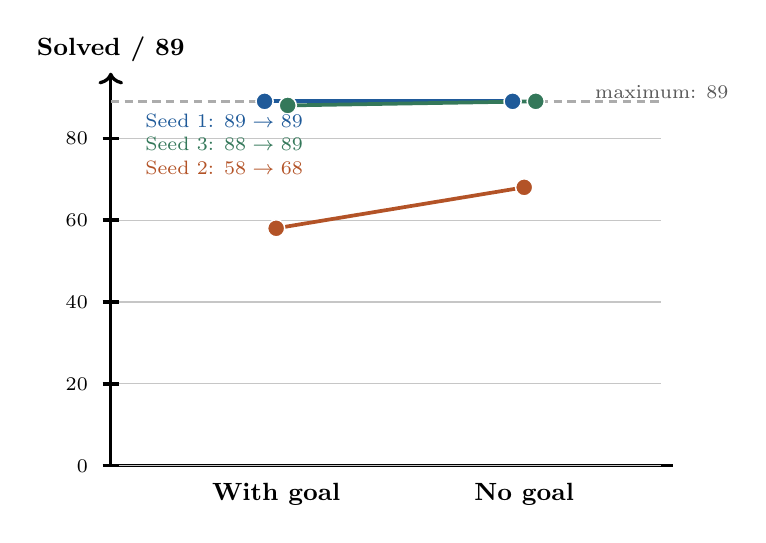
\begin{tikzpicture}[x=1.05cm,y=0.052cm]
  \definecolor{seedone}{HTML}{1F5A99}
  \definecolor{seedtwo}{HTML}{B35327}
  \definecolor{seedthree}{HTML}{34785A}

  \draw[->, very thick] (0,0) -- (0,96) node[above, font=\small\bfseries]{Solved / \good{}};
  \draw[very thick] (0,0) -- (6.8,0);
  \foreach \y in {0,20,40,60,80} {
    \draw[gray!45] (0,\y) -- (6.65,\y);
    \draw[very thick] (-0.10,\y) -- (0.10,\y);
    \node[left, font=\scriptsize] at (-0.16,\y) {\y};
  }
  \draw[densely dashed, line width=0.9pt, gray!65] (0,89) -- (6.65,89);
  \node[font=\scriptsize, text=gray!70!black, anchor=west] at (5.74,91.2) {maximum: 89};

  \node[font=\small\bfseries] at (2, -7.0) {With goal};
  \node[font=\small\bfseries] at (5, -7.0) {No goal};

  \draw[seedone, line width=1.35pt] (1.86,89) -- (4.86,89);
  \draw[seedtwo, line width=1.35pt] (2.00,58) -- (5.00,68);
  \draw[seedthree, line width=1.35pt] (2.14,88) -- (5.14,89);

  \filldraw[seedone, draw=white, line width=0.55pt] (1.86,89) circle (3.1pt);
  \filldraw[seedone, draw=white, line width=0.55pt] (4.86,89) circle (3.1pt);
  \filldraw[seedtwo, draw=white, line width=0.55pt] (2.00,58) circle (3.1pt);
  \filldraw[seedtwo, draw=white, line width=0.55pt] (5.00,68) circle (3.1pt);
  \filldraw[seedthree, draw=white, line width=0.55pt] (2.14,88) circle (3.1pt);
  \filldraw[seedthree, draw=white, line width=0.55pt] (5.14,89) circle (3.1pt);

  \node[font=\scriptsize, text=seedone, anchor=west] at (0.30,84.3) {Seed 1: $89 \rightarrow 89$};
  \node[font=\scriptsize, text=seedthree, anchor=west] at (0.30,78.6) {Seed 3: $88 \rightarrow 89$};
  \node[font=\scriptsize, text=seedtwo, anchor=west] at (0.30,72.9) {Seed 2: $58 \rightarrow 68$};

\end{tikzpicture}
\caption{Paired seed comparison for the goal-conditioning ablation: each line connects one seed's with-goal and no-goal solve count (out of \good{} meaningful problems), so slope shows the within-seed effect of removing the goal rather than an across-seed average. $\Delta$ is with-goal minus no-goal. Two of three seeds show a difference of $-1$ or $0$; the third shows $-10$. In both cases no-goal did not score lower.}
\label{fig:seeds}
\end{figure}

\Needspace{16\baselineskip}
We observed no consistent improvement from goal-conditioning across three paired seeds; the experiment is underpowered to exclude a smaller effect, and a benefit such as faster convergence or better sample efficiency would not necessarily show up in a fixed-budget, fixed-epoch comparison at all. A plausible mechanism: our benchmark's reference solutions are the \emph{unique} correct path in an otherwise heavily disambiguated corpus (Table~\ref{tab:branching} shows only two families ever offer a real alternative at all), so a policy that has learned "prefer the unwrapping move over the multiplying move" as a general prior can match a large fraction of reference paths without consulting an explicit goal token, provided its training data teaches that prior at sufficient depth and diversity. The training corpus includes a family, \texttt{goal-decides-distribute} (Section~\ref{sec:training}), constructed so this shortcut cannot work \emph{everywhere}; it is nonetheless sufficient to match goal-conditioned performance in aggregate on this benchmark, at this training budget. Isolating goal-conditioning's remaining contribution, if any, needs a larger seed count or a benchmark constructed so a state-only shortcut cannot exist at all.

\section{Limitations}
\label{sec:limitations}

\textbf{Scope.} \lemma{} covers seventeen template families in algebra, trigonometry, and linear equation solving. The results do not establish transfer to other mathematical domains, natural-language reasoning, or general theorem proving.

\textbf{Statistical power.} The ablation has three seeds per arm. That is enough to reject the earlier single-run interpretation, but not to estimate a small effect precisely. The v1/v2/v3 lineage (Appendix~\ref{sec:v-lineage}) has one run per arm and is descriptive rather than causal.

\textbf{Verifier scope.} Numerical verification samples a bounded number of points under a seeded generator; it is evidence, not proof, for identities the symbolic checker cannot close directly, and a pathological counterexample at unsampled points, while not observed in this work, is not excluded by construction.

\textbf{Comparison scope.} The benchmark compares decision procedures over a common verifier-admitted action space. It is not a cross-system leaderboard for computer algebra systems or theorem provers, which use different rule inventories and objectives.

\section{Conclusion}

On the frozen 89-problem decision-bearing benchmark, learned action guidance is sufficient for complete solution under greedy decoding. Uniform MCTS and value-only MCTS solve none of these problems; policy-only MCTS solves 87 and policy--value MCTS solves 61. Width-8 beam search rises from 0/89 at a 400 generated-successor cap to 28/89 at 800 and 89/89 at 1600. The controlled comparison therefore identifies the learned action policy as the most budget-efficient component in this setting: greedy decoding reaches the full corpus without tree search, while the present value head does not improve on it and beam requires a larger budget. The paired three-seed target-conditioning study finds no measured improvement from explicit target input under its evaluated protocol. Broader target-dependent and external evaluations remain important next tests of the same architecture.

\bibliographystyle{plainnat}
\begin{thebibliography}{9}

\bibitem[Meurer et al.(2017)]{sympy2017}
A.~Meurer, C.~P.~Smith, M.~Paprocki, O.~\v{C}ert\'{\i}k, S.~B.~Kirpichev, M.~Rocklin, A.~Kumar, S.~Ivanov, J.~K.~Moore, S.~Singh, T.~Rathnayake, S.~Vig, B.~E.~Granger, R.~P.~Muller, F.~Bonazzi, H.~Gupta, S.~Vats, F.~Johansson, F.~Pedregosa, M.~J.~Curry, A.~R.~Terrel, \v{S}.~Rou\v{c}ka, A.~Saboo, I.~Fernando, S.~Kulal, R.~Cimrman, A.~Scopatz.
\newblock SymPy: symbolic computing in Python.
\newblock \emph{PeerJ Computer Science}, 3:e103, 2017.

\bibitem[Silver et al.(2018)]{silver2018alphazero}
D.~Silver, T.~Hubert, J.~Schrittwieser, I.~Antonoglou, M.~Lai, A.~Guez, M.~Lanctot, L.~Sifre, D.~Kumaran, T.~Graepel, T.~Lillicrap, K.~Simonyan, D.~Hassabis.
\newblock A general reinforcement learning algorithm that masters chess, shogi, and Go through self-play.
\newblock \emph{Science}, 362(6419):1140--1144, 2018.

\bibitem[Polu and Sutskever(2020)]{polu2020gptf}
S.~Polu, I.~Sutskever.
\newblock Generative Language Modeling for Automated Theorem Proving.
\newblock \emph{arXiv:2009.03393}, 2020.

\bibitem[Lample et al.(2022)]{lample2022htps}
G.~Lample, T.~Lacroix, M.-A.~Lachaux, A.~Rodriguez, A.~Hayat, T.~Lavril, G.~Ebner, X.~Martinet.
\newblock HyperTree Proof Search for Neural Theorem Proving.
\newblock \emph{Advances in Neural Information Processing Systems (NeurIPS)}, 2022.

\bibitem[Willsey et al.(2021)]{egg2021}
M.~Willsey, C.~Nandi, Y.~R.~Wang, O.~Flatt, Z.~Tatlock, P.~Panchekha.
\newblock egg: Fast and Extensible Equality Saturation.
\newblock \emph{Proceedings of the ACM on Programming Languages}, 5(POPL), 2021.

\bibitem[Hubert et al.(2025)]{hubert2025alphaproof}
T.~Hubert, R.~Mehta, L.~Sartran, et al.
\newblock Olympiad-level formal mathematical reasoning with reinforcement learning.
\newblock \emph{Nature}, 2025.

\bibitem[Xie(2026)]{xie2026mathesis}
K.~Xie.
\newblock Constructing a Neuro-Symbolic Mathematician from First Principles.
\newblock \emph{arXiv:2601.00125}, 2026.

\bibitem[Lample and Charton(2020)]{lample2020symbolic}
G.~Lample, F.~Charton.
\newblock Deep Learning for Symbolic Mathematics.
\newblock \emph{International Conference on Learning Representations (ICLR)}, 2020. \emph{arXiv:1912.01412}.

\bibitem[Saxton et al.(2019)]{saxton2019mathematics}
D.~Saxton, E.~Grefenstette, F.~Hill, P.~Kohli.
\newblock Analysing Mathematical Reasoning Abilities of Neural Models.
\newblock \emph{arXiv:1904.01557}, 2019.

\bibitem[Charton(2022)]{charton2022linear}
F.~Charton.
\newblock Linear Algebra with Transformers.
\newblock \emph{Transactions on Machine Learning Research}, 2022. \emph{arXiv:2112.01898}.

\bibitem[d'Ascoli et al.(2022)]{dascoli2022symbolic}
S.~d'Ascoli, P.-A.~Kamienny, G.~Lample, F.~Charton.
\newblock Deep Symbolic Regression for Recurrent Sequences.
\newblock \emph{International Conference on Machine Learning (ICML)}, 2022. \emph{arXiv:2201.04600}.

\bibitem[Drori et al.(2022)]{drori2022neural}
I.~Drori, S.~Zhang, R.~Shuttleworth, L.~Tang, A.~Lu, E.~Ke, K.~Liu, L.~Chen, S.~Tran, N.~Cheng, R.~Wang, N.~Singh, T.~L.~Patti, J.~Lynch, A.~Shporer, N.~Verma, E.~Wu, G.~Strang.
\newblock A Neural Network Solves, Explains, and Generates University Math Problems by Program Synthesis and Few-Shot Learning at Human Level.
\newblock \emph{Proceedings of the National Academy of Sciences}, 119(32):e2123433119, 2022. \emph{arXiv:2112.15594}.

\bibitem[Davies et al.(2021)]{davies2021advancing}
A.~Davies, P.~Veli\v{c}kovi\'{c}, L.~Buesing, S.~Blackwell, D.~Zheng, N.~Toma\v{s}ev, R.~Tanburn, P.~Battaglia, C.~Blundell, A.~Juh\'{a}sz, M.~Lackenby, G.~Williamson, D.~Hassabis, P.~Kohli.
\newblock Advancing Mathematics by Guiding Human Intuition with AI.
\newblock \emph{Nature}, 600:70--74, 2021.

\bibitem[Knuth and Bendix(1970)]{knuthbendix1970}
D.~E.~Knuth, P.~B.~Bendix.
\newblock Simple Word Problems in Universal Algebra.
\newblock In J.~Leech (ed.), \emph{Computational Problems in Abstract Algebra}, pp.~263--297. Pergamon Press, 1970.

\bibitem[Dershowitz(1987)]{dershowitz1987termination}
N.~Dershowitz.
\newblock Termination of Rewriting.
\newblock \emph{Journal of Symbolic Computation}, 3(1--2):69--116, 1987.

\bibitem[Baader and Nipkow(1998)]{baadernipkow1998term}
F.~Baader, T.~Nipkow.
\newblock \emph{Term Rewriting and All That}.
\newblock Cambridge University Press, 1998.

\bibitem[Bezem et al., eds.(2003)]{terese2003term}
M.~Bezem, J.~W.~Klop, R.~de Vrijer, eds. (``Terese'').
\newblock \emph{Term Rewriting Systems}.
\newblock Cambridge Tracts in Theoretical Computer Science 55. Cambridge University Press, 2003.

\bibitem[Visser(2001)]{visser2001stratego}
E.~Visser.
\newblock Stratego: A Language for Program Transformation Based on Rewriting Strategies (System Description of Stratego 0.5).
\newblock \emph{Rewriting Techniques and Applications (RTA)}, LNCS 2051, pp.~357--362. Springer, 2001.

\bibitem[Clavel et al.(2002)]{clavel2002maude}
M.~Clavel, F.~Dur\'{a}n, S.~Eker, P.~Lincoln, N.~Mart\'{\i}-Oliet, J.~Meseguer, J.~F.~Quesada.
\newblock Maude: Specification and Programming in Rewriting Logic.
\newblock \emph{Theoretical Computer Science}, 285(2):187--243, 2002.

\bibitem[Tate et al.(2009)]{tate2009equality}
R.~Tate, M.~Stepp, Z.~Tatlock, S.~Lerner.
\newblock Equality Saturation: A New Approach to Optimization.
\newblock \emph{Proceedings of the 36th ACM SIGPLAN-SIGACT Symposium on Principles of Programming Languages (POPL)}, pp.~264--276, 2009.

\bibitem[Nandi et al.(2021)]{nandi2021ruler}
C.~Nandi, M.~Willsey, A.~Zhu, Y.~R.~Wang, B.~Saiki, A.~Anderson, A.~Schulz, D.~Grossman, Z.~Tatlock.
\newblock Rewrite Rule Inference Using Equality Saturation.
\newblock \emph{Proceedings of the ACM on Programming Languages}, 5(OOPSLA), 2021. \emph{arXiv:2108.10436}.

\bibitem[Gauthier et al.(2021)]{gauthier2021tactictoe}
T.~Gauthier, C.~Kaliszyk, J.~Urban, R.~Kumar, M.~Norrish.
\newblock TacticToe: Learning to Prove with Tactics.
\newblock \emph{Journal of Automated Reasoning}, 65(2):257--286, 2021. \emph{arXiv:1804.00596}.

\bibitem[Bansal et al.(2019a)]{bansal2019holist}
K.~Bansal, S.~M.~Loos, M.~N.~Rabe, C.~Szegedy, S.~Wilcox.
\newblock HOList: An Environment for Machine Learning of Higher-Order Theorem Proving.
\newblock \emph{International Conference on Machine Learning (ICML)}, 2019. \emph{arXiv:1904.03241}.

\bibitem[Bansal et al.(2019b)]{bansal2019deephol}
K.~Bansal, C.~Szegedy, M.~N.~Rabe, S.~M.~Loos, V.~Toman.
\newblock Learning to Reason in Large Theories without Imitation.
\newblock \emph{arXiv:1905.10501}, 2019.

\bibitem[Yang and Deng(2019)]{yang2019coqgym}
K.~Yang, J.~Deng.
\newblock Learning to Prove Theorems via Interacting with Proof Assistants.
\newblock \emph{International Conference on Machine Learning (ICML)}, 2019. \emph{arXiv:1905.09381}.

\bibitem[Han et al.(2021)]{han2021pact}
J.~M.~Han, J.~Rute, Y.~Wu, E.~W.~Ayers, S.~Polu.
\newblock Proof Artifact Co-training for Theorem Proving with Language Models.
\newblock \emph{International Conference on Learning Representations (ICLR)}, 2021. \emph{arXiv:2102.06203}.

\bibitem[Wu et al.(2021)]{wu2021tacticzero}
M.~Wu, M.~Norrish, C.~Walder, A.~Dezfouli.
\newblock TacticZero: Learning to Prove Theorems from Scratch with Deep Reinforcement Learning.
\newblock \emph{Advances in Neural Information Processing Systems (NeurIPS)}, 2021. \emph{arXiv:2102.09756}.

\bibitem[Jiang et al.(2022)]{jiang2022thor}
A.~Q.~Jiang, W.~Li, S.~Tworkowski, K.~Czechowski, T.~Odrzyg\'{o}\'{z}d\'{z}, P.~Mi\l{}o\'{s}, Y.~Wu, M.~Jamnik.
\newblock Thor: Wielding Hammers to Integrate Language Models and Automated Theorem Provers.
\newblock \emph{arXiv:2205.10893}, 2022.

\bibitem[Yang et al.(2023)]{yang2023leandojo}
K.~Yang, A.~M.~Swope, A.~Gu, R.~Chalamala, P.~Song, S.~Yu, S.~Godil, R.~Prenger, A.~Anandkumar.
\newblock LeanDojo: Theorem Proving with Retrieval-Augmented Language Models.
\newblock \emph{Advances in Neural Information Processing Systems (NeurIPS), Datasets and Benchmarks Track}, 2023. \emph{arXiv:2306.15626}.

\bibitem[First et al.(2023)]{first2023baldur}
E.~First, M.~N.~Rabe, T.~Ringer, Y.~Brun.
\newblock Baldur: Whole-Proof Generation and Repair with Large Language Models.
\newblock \emph{Proceedings of the 31st ACM Joint European Software Engineering Conference and Symposium on the Foundations of Software Engineering (ESEC/FSE)}, 2023. \emph{arXiv:2303.04910}.

\bibitem[Jiang et al.(2021)]{jiang2021lisa}
A.~Q.~Jiang, W.~Li, J.~M.~Han, Y.~Wu.
\newblock LISA: Language Models of Isabelle Proofs.
\newblock \emph{6th Conference on Artificial Intelligence and Theorem Proving (AITP)}, 2021.

\bibitem[Blum and Kannan(1995)]{blum1995designing}
M.~Blum, S.~Kannan.
\newblock Designing Programs that Check Their Work.
\newblock \emph{Journal of the ACM}, 42(1):269--291, 1995.

\bibitem[McConnell et al.(2011)]{mcconnell2011certifying}
R.~M.~McConnell, K.~Mehlhorn, S.~N\"{a}her, P.~Schweitzer.
\newblock Certifying Algorithms.
\newblock \emph{Computer Science Review}, 5(2):119--161, 2011.

\bibitem[Alkassar et al.(2014)]{alkassar2014framework}
E.~Alkassar, S.~B\"{o}hme, K.~Mehlhorn, C.~Rizkallah.
\newblock A Framework for the Verification of Certifying Computations.
\newblock \emph{Journal of Automated Reasoning}, 52(3):241--273, 2014. \emph{arXiv:1301.7462}.

\bibitem[Harrison and Th\'{e}ry(1998)]{harrison1998skeptic}
J.~Harrison, L.~Th\'{e}ry.
\newblock A Skeptic's Approach to Combining HOL and Maple.
\newblock \emph{Journal of Automated Reasoning}, 21(3):279--294, 1998.

\bibitem[Kaliszyk and Wiedijk(2007)]{kaliszyk2007certified}
C.~Kaliszyk, F.~Wiedijk.
\newblock Certified Computer Algebra on Top of an Interactive Theorem Prover.
\newblock \emph{Towards Mechanized Mathematical Assistants (MKM/Calculemus)}, LNCS 4573, pp.~94--105. Springer, 2007.

\bibitem[Th\'{e}ry(2001)]{thery2001buchberger}
L.~Th\'{e}ry.
\newblock A Machine-Checked Implementation of Buchberger's Algorithm.
\newblock \emph{Journal of Automated Reasoning}, 26(2):107--137, 2001.

\bibitem[Harrison(2008)]{harrison2008formal}
J.~Harrison.
\newblock Formal Proof: Theory and Practice.
\newblock \emph{Notices of the American Mathematical Society}, 55(11):1395--1406, 2008.

\bibitem[Trinh et al.(2024)]{trinh2024alphageometry}
T.~H.~Trinh, Y.~Wu, Q.~V.~Le, H.~He, T.~Luong.
\newblock Solving Olympiad Geometry without Human Demonstrations.
\newblock \emph{Nature}, 625:476--482, 2024.

\bibitem[Romera-Paredes et al.(2024)]{romeraparedes2024funsearch}
B.~Romera-Paredes, M.~Barekatain, A.~Novikov, M.~Balog, M.~P.~Kumar, E.~Dupont, F.~J.~R.~Ruiz, J.~S.~Ellenberg, P.~Wang, O.~Fawzi, P.~Kohli, A.~Fawzi.
\newblock Mathematical Discoveries from Program Search with Large Language Models.
\newblock \emph{Nature}, 625:468--475, 2024.

\bibitem[Novikov et al.(2025)]{novikov2025alphaevolve}
A.~Novikov, N.~V\~{u}, M.~Eisenberger, E.~Dupont, P.-S.~Huang, A.~Z.~Wagner, S.~Shirobokov, B.~Kozlovskii, F.~J.~R.~Ruiz, A.~Mehrabian, M.~P.~Kumar, A.~See, S.~Chaudhuri, G.~Holland, A.~Davies, S.~Nowozin, P.~Kohli, M.~Balog.
\newblock AlphaEvolve: A Coding Agent for Scientific and Algorithmic Discovery.
\newblock \emph{arXiv:2506.13131}, 2025.

\bibitem[Poesia and Goodman(2023)]{poesia2023peano}
G.~Poesia, N.~D.~Goodman.
\newblock Peano: Learning Formal Mathematical Reasoning.
\newblock \emph{Philosophical Transactions of the Royal Society A}, 381(2251), 2023. \emph{arXiv:2211.15864}.

\bibitem[Qin et al.(2021)]{qin2021nssolver}
J.~Qin, X.~Liang, Y.~Hong, J.~Tang, L.~Lin.
\newblock Neural-Symbolic Solver for Math Word Problems with Auxiliary Tasks.
\newblock \emph{Proceedings of the 59th Annual Meeting of the Association for Computational Linguistics (ACL-IJCNLP)}, pp.~5870--5881, 2021. \emph{arXiv:2107.01431}.

\end{thebibliography}

\appendix
\section{The v1/v2/v3 Lineage}
\label{sec:v-lineage}

v1, v2, and v3 differ in more than one respect, including training data breadth, encoder width, and whether off-path recovery examples were included. Each is a single training run, so we do not treat them as a matched study the way Section~\ref{sec:ablation} is. We isolated the recovery-data variable directly: v3 is v2's exact architecture, training data, and hyperparameters with \texttt{--recovery-per-problem 0}, and its \good{}-problem score (61) is close to v1's (59) and well above v2's (32), the run that included recovery data. We report this as a genuine, single-run finding worth further investigation. In this particular training configuration, recovery data correlated with lower rather than higher solve rate, and we explicitly do not claim it as an established causal effect, since establishing that would need the same seed-matched treatment Section~\ref{sec:ablation} gives goal-conditioning.

\subsection{Why v2's validation accuracy did not predict its solve rate}
\label{sec:v2-gap}

v2 reached 100\% legal-action top-1 accuracy on its own held-out validation split by epoch 1, yet solved only 32 of \good{} meaningful benchmark problems (Table~\ref{tab:headline}). This is the largest validation/benchmark gap of any arm in this paper, and one worth explaining rather than reporting as a curiosity. We measured v2's actual per-state top-1 accuracy directly on the frozen benchmark corpus (not its own training-distribution validation split) by replaying each benchmark problem's reference path and checking whether the policy's top legal-action prediction matches the reference rule at every state, on small stratified samples (11 \texttt{identity} problems, 1,344 states; 2 \texttt{power\_of\_one} problems, 128 states) chosen to avoid contending for CPU with the budget-curve experiment (Appendix~\ref{sec:budget-curve}) running concurrently.

The result does not have one clean explanation. For \texttt{power\_of\_one}, measured per-state accuracy is 98.39\%, but naive compounding ($p^{\text{depth}}$) already predicts only 35\%/21\%/13\% success at depths 64/96/128, which is consistent with the observed collapse to 0/29, though the true failure is total while the naive arithmetic is not, plausibly because MCTS must also \emph{find} the correct branch at a near-50/50 decision (Table~\ref{tab:branching}) at every one of up to 128 levels, a second bottleneck beyond raw policy accuracy. For \texttt{identity}, this explanation fails outright: measured per-state accuracy is 100\% in every one of the 1,344 sampled states, yet only 32 of 60 \texttt{identity} problems (53\%) are solved, falling with depth despite constant per-step accuracy. Compounding a 100\% rate predicts near-total success, not 53\%.

A second mechanism better fits \texttt{identity}: v2's train/validation split (\texttt{split\_problems} in \texttt{train\_goal\_deep.rs}) holds out whole problems stratified by depth and family, but not by wrapper-motif \emph{composition}. Training's composition layer draws each wrapper motif independently from a seven-way distribution (Section~\ref{sec:training}), so a problem with roughly 63 consecutive identity-collision layers, the benchmark's actual construction, has probability on the order of $0.24^{63} \approx 0$ under training's own distribution, even though the atomic identity-collision motif itself is common (24\% of layers). The benchmark's monotone-repeat composition is close to unseen during training despite sharing motif vocabulary with it, which is a more specific claim than the deep-OOD legacy-naming issue of Section~\ref{sec:setup} and applies even to the \texttt{deep-ID} split. We read this as the more likely explanation for why a policy with a measured-correct prior at every sampled state still fails to convert that into a solved long-horizon problem: most plausibly, MCTS's fixed simulation budget cannot accumulate enough confidence margin to commit to the correct branch when the training distribution never rehearsed this specific compositional shape, even though it rehearsed every component of it.

Both measurements use small samples (11 and 2 problems respectively) and should be read as suggestive point estimates, not precise population values. The result is family-dependent and unresolved: compounding error accounts for \texttt{power\_of\_one}'s collapse but not \texttt{identity}'s, and we report both rather than only the mechanism that fits.

\section{Reproducibility Details}
\label{sec:repro}

The source code, training and evaluation harness, and paper artifacts are available in the \href{https://github.com/blackdromeai-labs/LEMMA}{GitHub repository}. The frozen benchmark is released as a \href{https://huggingface.co/datasets/BlackdromeAILabs/lemma-long-horizon-rewrite-benchmark}{Hugging Face dataset}; the paper's 120-problem evaluation uses its \texttt{deep} configuration. The evaluated checkpoint is released as the \href{https://huggingface.co/BlackdromeAILabs/lemma-v3-policy}{LEMMA v3 policy model}. The archival paper record is available at \href{https://doi.org/10.5281/zenodo.22842820}{doi:10.5281/zenodo.22842820}.

\subsection{Arms evaluated}
Table~\ref{tab:arms} lists every arm referenced in this paper together with its training configuration, for exact reproduction.

\begin{table}[H]
\centering
\small
\begin{tabular}{@{}llll@{}}
\toprule
Arm & Guidance & Recovery data & Goal-conditioned \\
\midrule
Uniform prior & none & n/a & n/a \\
Shallow template policy & template, 1-step & n/a & no \\
Compositional template policy & template, compositional & n/a & no \\
Trained, v1 & learned & yes & yes \\
Trained, v2 & learned & yes & yes \\
Trained, v3 & learned & no & yes \\
Ablation, with-goal (3 seeds) & learned & no & yes \\
Ablation, no-goal (3 seeds) & learned & no & no \\
\bottomrule
\end{tabular}
\caption{Full arm inventory.}
\label{tab:arms}
\end{table}

\subsection{Network and search hyperparameters}
Embedding dimension 256, hidden dimension 512, 8 attention heads, 4 transformer layers, token vocabulary 64, dropout 0.1 during training, \textbf{2{,}272{,}318 parameters across 69 tensors} (counted directly from a saved checkpoint, not estimated). Optimizer: AdamW, weight decay 0.01. Value loss weight 0.5. Cosine learning-rate schedule, peak $3\times10^{-4}$, minimum $3\times10^{-5}$, warmup 5\% of total steps. Value-target discount 0.97. Checkpoint selection: every epoch's weights are saved unconditionally to the primary output path (Section~\ref{sec:training}), so the file on disk after training is the \emph{last} epoch run, not the epoch with the best validation metric; early stopping triggers once \texttt{min\_epochs} (12, or as noted per arm below) has elapsed and \texttt{patience} (6) further epochs pass with no improvement in branching-validation accuracy.

MCTS exploration constant $c_{\text{puct}}=1.41$; evaluation simulation budget 400 per problem (except the budget sweep, Appendix~\ref{sec:budget-curve}); maximum search depth is the deepest benchmark problem's construction depth plus 8. Backup is a simple running mean of backed-up values per node ($\texttt{visits} \mathrel{+}= 1$, $\texttt{value\_sum} \mathrel{+}= v$), not a discounted or minimax backup. Reaching the goal predicate backs up a fixed terminal value of $1.0$; every other leaf (expansion, max-depth cutoff, or no legal moves) backs up the trained value head's prediction. Final action extraction is deterministic, not temperature-sampled: if any goal-reaching path exists in the tree, the shortest one is taken; otherwise the most-visited child is followed at each step, ties broken toward the lower action index. No Dirichlet or other exploration noise is added to the root priors. Exploration is driven only by PUCT's own $c_{\text{puct}} \cdot P(s,a) \cdot \sqrt{N(s)}/(1+N(s,a))$ term.

\subsection{Per-arm training data and wall time}
Table~\ref{tab:training-config} reports what each run's own manifest actually recorded; a blank cell means that field was not logged for that specific run rather than being assumed zero or omitted for space. All arms share the network and optimizer settings above; \texttt{--recovery-per-problem} and per-depth problem count are the two training-recipe parameters that differ across arms (Table~\ref{tab:arms}).

\begin{table}[h]
\centering
\scriptsize
\resizebox{\textwidth}{!}{%
\begin{tabular}{@{}lrrrrr@{}}
\toprule
Arm & Problems validated & Training rows (nominal $\to$ distinct) & On-path / recovery & Epochs run & Wall time \\
\midrule
v1 & 2{,}458 & 91{,}110 $\to$ 66{,}754 & 78{,}874 / 12{,}236 & 13 & 7{,}733.5s \\
v2 & 1{,}099 & 46{,}107 $\to$ 43{,}462 & 44{,}497 / 1{,}610 & n/a & 7{,}812.4s \\
v3 & 1{,}099 & 44{,}497 $\to$ 42{,}520 & 44{,}497 / 0 & 7 & 2{,}398.9s \\
Ablation, with/no-goal (each seed) & 549 & 22{,}247 $\to$ 21{,}408--21{,}432 & 22{,}247 / 0 & 4 & 510--642s \\
\bottomrule
\end{tabular}%
}
\caption{Per-arm training statistics, taken directly from each run's own saved manifest. v1's epoch count is inferred from its best-epoch report (epoch 12, zero-indexed) rather than separately logged; v2's total epoch count was not captured in its manifest. Ablation wall times vary slightly by seed at fixed epoch count due to normal machine-load variation, not a configuration difference.}
\label{tab:training-config}
\end{table}

Evaluation runtime: the full 120-problem frozen corpus at 400 simulations takes approximately 12 minutes per arm on the parallelized evaluator (roughly seven times faster than the original sequential implementation, Section~\ref{sec:setup}) on a 16-logical-core workstation CPU.

\subsection{Seeds}
Training data generation seed and evaluation corpus generation seed are independently frozen and distinct. Distinct seeds alone do not guarantee zero overlap: an explicit check compares every generated training input against the held-out corpora by exact string match and discards a collision before it can reach a training example. This check is not vacuous. It caught and removed one exact collision during v2's data generation, so it is the filter, not the seed choice, that rules out train/test leakage. The ablation study's per-seed weight-initialization and batch-order seed is an explicit, logged command-line argument (Section~\ref{sec:seed-bug}); the train/validation split and the underlying training data are held fixed across seeds within an arm.

\section{Solve Rate versus Simulation Budget}
\label{sec:budget-curve}

The main text (Section~\ref{sec:headline}) reports every arm at a single simulation budget (400) and is explicit that it does not characterize how solve rate scales with budget. Table~\ref{tab:budget} closes that gap for one arm, v3, at five budgets from 50 to 800.

\begin{table}[H]
\centering
\small
\begin{tabular}{@{}rrrrr@{}}
\toprule
Simulations & Total (/120) & \texttt{identity} (/60) & \texttt{power\_of\_one} (/29) & Meaningful (/\good{}) \\
\midrule
50  & 0  & 0  & 0  & 0 \\
100 & 45 & 14 & 8  & 22 \\
200 & 84 & 36 & 17 & 53 \\
400 & 92 & 44 & 17 & 61 \\
800 & 96 & 48 & 17 & 65 \\
\bottomrule
\end{tabular}
\caption{v3's solve rate against simulation budget, on the same frozen corpus and wrapper-family classification as Table~\ref{tab:headline}. The 400-simulation row (61/\good{}) matches the main text exactly, run independently on the parallelized evaluator (Section~\ref{sec:setup}) as a consistency check.}
\label{tab:budget}
\end{table}

Two things follow. First, guidance alone is not sufficient at every budget: v3 solves \emph{zero} meaningful problems at 50 simulations despite being the same trained policy that solves 61 of them at 400. A search budget too small to realize a correct policy's advantage looks, from the outside, identical to having no useful policy at all. Second, returns diminish but do not vanish by 800: \texttt{power\_of\_one} is flat at 17/29 from 200 simulations onward (its remaining 12 problems are not solved by more search at this policy's fixed accuracy, consistent with Appendix~\ref{sec:v2-gap}'s compounding-error analysis), while \texttt{identity} continues to improve through 800 (48/60, up from 44/60 at 400). We did not extend the sweep past 800 simulations; whether \texttt{identity}'s improvement continues, plateaus, or reflects a budget large enough to overcome the compositional-mismatch effect of Appendix~\ref{sec:v2-gap} is not established by this experiment.

\end{document}
